\documentclass[journal]{IEEEtran}

\usepackage{amsmath,amsfonts,amssymb}
% \usepackage{algorithmic}
% \usepackage{array}
% \usepackage{textcomp}
% \usepackage{stfloats}
\usepackage{graphicx}
% \usepackage{xcolor}
% \usepackage{xspace}
% \usepackage{booktabs}
\usepackage{authblk}
\usepackage{url}
\usepackage{hyperref}
\usepackage{placeins}
\usepackage{caption}
\usepackage{subfigure}
\usepackage[maxcitenames=3,natbib=true,giveninits=true,backend=bibtex]{biblatex}
\addbibresource{bibliography.bib}
\usepackage{microtype}

\usepackage{booktabs} % for professional tables
\def\BibTeX{{\rm B\kern-.05em{\sc i\kern-.025em b}\kern-.08em
    T\kern-.1667em\lower.7ex\hbox{E}\kern-.125emX}}
\usepackage{balance}

\DeclareMathOperator*{\argmin}{arg\,min}
\DeclareMathOperator*{\argmax}{arg\,max}
\DeclareMathOperator*{\minimise}{\textrm{minimise}}
\DeclareMathOperator*{\maximise}{\textrm{maximise}}

\begin{document}
\title{A Training Rate and Survival Heuristic for Inference and Robustness Evaluation (TRASHFIRE)}
\author[1]{Charles Meyers}
\author[2]{Mohammad Reza Saleh Sedghpour}
\author[1]{Tommy L\"{o}fstedt}
\author[1]{Erik Elmroth}
\affil[1]{Department of Computing Science, Ume{\aa} University, {Ume\aa}, Sweden}
\affil[2]{Elastisys AB}


\maketitle


\begin{abstract}
%  Big Topic Intro
Machine learning models---deep neural networks in particular---have performed remarkably well on benchmark datasets across a wide variety of domains. However, the ease of finding adversarial counter-examples remains a persistent problem when training times are measured in hours or days and the time needed to find a successful adversarial counter-example is measured in seconds.
%  Problem Statement and Drawbacks
Much work has gone into generating and defending against these adversarial counter-examples, however the relative costs of attacks and defences are rarely discussed. Additionally, machine learning research is almost entirely guided by test/train metrics, but these would require billions of samples to meet industry standards. The present work addresses the problem of understanding and predicting how particular model hyper-parameters influence the performance of a model in the presence of an adversary.
%  Our solution and Advantages of our solution
The proposed approach uses survival models, worst-case examples, and a cost-aware analysis to precisely and accurately reject a particular model change during routine model training procedures rather than relying on real-world deployment, expensive formal verification methods, or accurate simulations of very complicated systems (\textit{e.g.}, digitally recreating every part of a car or a plane).
%  Conclusion  TODO quantify or examplify this somehow?
Through an evaluation of many pre-processing techniques, adversarial counter-examples, and neural network configurations, the conclusion is that deeper models do offer marginal gains in survival times compared to more shallow counterparts. However, we show that those gains are driven more by the model inference time than inherent robustness properties. Using the proposed methodology, we show that ResNet is hopelessly insecure against even the simplest of white box attacks.
\end{abstract}
\section{Introduction}

Machine Learning (ML) has become a widely popular tool for solving complex problems across many disciplines, like medical imaging (\citep{}). Despite this, adversarial attacks aim to exploit vulnerabilities in machine learning models by introducing subtle modifications to data submitted to various stages of the ML pipeline, leading to misclassification or otherwise erroneous outputs~\citep{chakraborty_adversarial_2018}. Ensuring the robustness of ML models against adversaries has become a critical concern~\citep{adversarialpatch,carlini_towards_2017,croce_reliable_2020,hopskipjump,art2018,meyers}. However, understanding the relationship between computational cost and the performance against adversarial noise remains an ongoing challenge.  In this paper, we  investigate the robustness of various deep neural networks and data pre-processing techniques against adversarial attacks and explore the relationship between computational cost and  prediction accuracy in both benign and adversarial contexts.  By using samples crafted specifically to be challenging and applying accelerated failure rate models (see Sec.~\ref{afr_models}) we provide a way to estimate the expected failure time across the entire feasible adversarial space. Using this model, we demonstrate that larger models, while offering marginal gains over smaller models, do so at the expense of training times that far outpace the expected adversarial training time.

\subsection{Contributions}

We summarize our contributions below:
\begin{itemize}
    \item We propose to use accelerated failure time methods for analyzing ML models under adversarial perturbations and provide substantial empirical evidence that this method is both effective and dataset-agnostic, allowing us to predict the expected failure rate more precisely and accurately than with either adversarial or benign accuracy alone.
    \item We use this method to measure model robustness across a wide variety of signal pre-processing techniques to explore the relationships between latency, up-time, accuracy, and model depth.
    \item We use this method to show that, at best, increasing the number of hidden layers in a neural network increases training time while having little-to-no benefit in the presence of an adversary.
\end{itemize}

\section{Background}
Much work has gone into explaining the dangers of adversarial attacks on ML pipelines~\cite{carlini_towards_2017,croce_reliable_2020,pixelattack,fgm,biggio_evasion_2013}, though studies on adversarial robustness have generally been limited to ad-hoc and posterior evaluations against limited sets of attack and defence parameters, leading to results that are, at best, optimistic~\cite{meyers,ma2020imbalanced}. Previous work on neural network verification have relied on expensive integration tests~\cite{vehicle_testing_review}, elaborate simulation environments~\cite{vehicle_formal}, or methods that are too computationally expensive to be useful for model selection~\cite{formal_adversarial}.
However, the present work formalises methods to model the effect of attacks and defences on a given ML model and reveals a simple cost-to-performance metric to quickly discard ineffective strategies.

\subsection{Adversarial Attacks}
In the context of ML, an adversarial attack refers to deliberate and malicious attempts to manipulate the behaviour of a model. The presented work focuses on \textit{evasion attacks} that attempt to induce misclassifications at run-time~\cite{carlini_towards_2017,biggio_evasion_2013}, but note that the proposed methodology (Section~\ref{aft_models}) and cost analysis (Section~\ref{cost_normalization}) extends to other types of attacks, such as database poisoning~\cite{biggio_poisoning_2013,saha2020hidden}, model inversion~\cite{choquette2021label,li2021membership}, data stealing~\cite{orekondy2019knockoff}, or denial of service~\cite{santos2021universal}. In all sections below, metrics were collected on the benign (unperturbed) data and adversarial (perturbed) data. The abbreviations \textit{ben} and \textit{adv} are used throughout, respectively.
The strength of an attack is often measured in terms of a perturbation distance~\cite{croce_reliable_2020,chakraborty_adversarial_2018,pixelattack}. The perturbation distance, denoted by $\varepsilon\geq0$, quantifies the magnitude of the perturbation applied to a sample, $x$, when generating a new adversarial sample, $x'$. The definition is,
\begin{equation}
    \varepsilon := \| x' - x \| \leq \varepsilon^*,
    \label{eq:perturbation_distance}
\end{equation}
where $\| \cdot \|$ denotes a norm or pseudo-norm (\textit{e.g.}, the Euclidean $\ell_2$ norm or the $\ell_0$ pseudo-norm). We denote by $\varepsilon^*$ the maximum allowed perturbation of the original input. For example, this might be one bit, one pixel, or one byte, depending on the test conditions. For more information on different criteria, see Section~\ref{attacks}.


\subsubsection{Accuracy and Failure Rate}
The accuracy refers to the percentage or proportion of examples that are correctly classified. A lower accuracy indicates a higher rate of misclassifications or incorrect predictions. The accuracy, $\mathrm{Acc}$, is defined as
\begin{equation}
    \mathrm{Acc} := 1 - \frac{\mathrm{False~Classifications}}{N},
    \label{eq:acc}
\end{equation}
where $N$ is the total number of samples. The accuracy on a given test set, presumed to be drawn from the same distribution as the training set, is called the \textit{benign accuracy}, $\mathrm{Acc}_{\mathrm{ben}}$. The \textit{adversarial accuracy}, $\mathrm{Acc}_{\mathrm{adv}}$, is a measure of correct classifications in the presence of noise intended to be adversarial. However, accuracy is known to vary with things like model complexity~\cite{vgg,resnet}, data resolution~\cite{feature_squeezing}, the number of samples~\cite{vapnik1994measuring}, the number of classes~\cite{dohmatob_generalized_2019}, or the amount of noise in the data~\cite{gauss_aug,gauss_out,dohmatob_generalized_2019}. Many of these factors can also influence an attack's run time. For this reason, it is useful to think in terms of \textit{failure rate}, as
\begin{equation}
    \mathrm{Failure~Rate} := \frac{\mathrm{False~Classifications}}{\Delta t} ,
    \label{eq:failure_rate}
\end{equation}
where $\Delta t$ is a time interval. By parameterizing the measure of misclassification by time, it is possible to model the chance of failure as a function of various attributes and parameters of a model.

Let $h$ be a function that describes the rate of failure at time $t$.
This is a way to express the failure rate in terms of a \textit{hazard function}, which is defined as
\begin{equation}
    h(t) := \lim_{ \Delta t \rightarrow 0} \frac{P(t \leq T < t + \Delta t \,|\, T \geq t)}{\Delta t},
    \label{eq:failure_rate_h}
\end{equation}
where  $P(\cdot)$ is a probability and $T$ is the time until a false classification occurs, also referred to as \textit{survival time}~\cite{kleinbaum1996survival}. To be able to compare the computational efficacy of different model and attack configurations, we modelled the probability of not observing a failure before a given time, $t$, using the \textit{cumulative hazard function},
\begin{equation}
     H(t) := \int_0^{t} h(\tau) \,d\tau.
     \label{eq:cdf}
\end{equation}
Then, the \textit{cumulative survival function} is
\begin{equation}
    S(t) := P(T \geq t) = \exp(-H(t)) = 1 - F(t) = 1-   \int_0^t f(u)du
    \label{eq:S(t)}
\end{equation}
where $F(t)$ is the \textit{lifetime distribution function} which describes the cumulative probability of failure before time $t$, or $F(t) = P(T < t)$.
The probability density of observing a failure at time, $t$, is~\cite{kleinbaum1996survival},
\begin{equation*}
    f(t) := h(t)S(t).
    \label{eq:pdf}
\end{equation*}
In practice, the $h(t), S(t)$, and/or $f(t)$ can be determined whenever one of them is known~\cite{kleinbaum1996survival}.

\subsection{Cost}
\label{cost}

Assume that the cost of training a model, $C_{\mathrm{train}}$, is a function of the total training time, $T_{\mathrm{train}}$, the number of training samples, $N_{\mathrm{train}}$, and the training time per sample, $t_{\mathrm{train}} = \frac{T_{\mathrm{train}}}{N_{\mathrm{train}}}$, such that the cost of training on hardware with a fixed time-cost is
\begin{equation}
    C_{\mathrm{train}} := C_{h} \cdot T_{\mathrm{train}} = C_h \cdot t_{\mathrm{train}} \cdot N_{\mathrm{train}},
    \label{eq:naive_cost}
\end{equation}
where $C_h$ is the cost per time unit of a particular piece of hardware. Hence, the cost is assumed to scale linearly with per-sample training time and sample size, $N_{\mathrm{train}}$.
Analogously, $t_{\mathrm{predict}}$ is used elsewhere in this text to refer to the prediction time for a set of samples, divided by the number of samples. Assuming the attacker and model builder are using similar hardware then the cost to an attacker, $C_{\mathrm{attack}}$, is
\[
    C_{\mathrm{attack}} := C_{h} \cdot T_{\mathrm{attack}} = C_h \cdot t_{\mathrm{attack}} \cdot N_{\mathrm{attack}},
\]
where $ N_{\mathrm{attack}} $ is the number of attacked samples. Furthermore, a fast attack will be lower-bounded by the model inference time, $ t_{\mathrm{predict}} $, which is generally much smaller than the training time, $ t_{\mathrm{train}} $. Of course, the long-term costs of deploying a model will be related to the inference cost, but a model is clearly broken if the cost of improving a model ($\propto t_{\mathrm{train}}$) is larger than the cost of finding a counterexample ($\propto t_{\mathrm{attack}}$) within the bounds outlined in Equation~\ref{eq:perturbation_distance}. The training cost per sample does not consider how well the model performs, and a good model is one that both generalises and is reasonably cheap to train.
Therefore, a cost-normalised failure rate metric is introduced in Equation~\ref{eq:cost} in Section~\ref{cost_normalization}. Before comparing this cost to the failure rate, the attack time per sample -- or the expected survival time --  must be estimated. For that, survival models can be used.

\section{Survival Analysis for ML} 
\label{afr_models}

Failure time analysis has been widely explored in other fields~\cite{aft_models}, from medicine to industrial quality control~\cite{ai_medical_imaging,ai_industry,ai_aviation,ai_luggage,ai_security,ai_prison}, but there is very little published research in the context of ML. However, as noted by many researchers~\cite{madry2017towards, carlini_towards_2017, croce_reliable_2020, meyers}, these models are fragile to attackers that intend to subvert the model, steal the database, or evade detection.  \cm{In this work, we leverage evasion attacks to examine the parameterised time-to-failure -- or survival time -- denoted $S_{\theta}(t)$, where $\theta$ is a set of parameters that describe the joint effect of the covariates on the survival time, usually found through maximum likelihood estimation on observed survival data~\cite{collett2023modelling}.} All survival models can be expressed in terms of this parameterised survival function, $S_\theta(t)$, hazard function, $H_\theta(t)$, and lifetime probability distribution, $F_{\theta}(t)$, such that
$$
	S_{\theta}(t) := \exp\big\{-H_{\theta}(t)\big\} := 1 - F_{\theta}(t) := 1 - \int_0^t f_\theta(u) du,
$$
and the expected survival time is thus
$$
	\mathbb{E}_{S_\theta}[T] =  \int_{0}^{t^*} S_{\theta}(u) du \approx t_{\mathrm{attack}}, 
$$
where $t_{\mathrm{attack}}$ is an estimate of the time it takes for the average attacker to induce a failure subject to the condition in Equation~\ref{eq:perturbation_distance} \cm{and $t^*$ is the latest observed time (regardless of failure or success)}. The parameters, $\theta$, are estimated from model evaluation data such that: $h_{\theta}(t=t_{attack}) \approx 1 - \mathrm{Acc}_{\mathrm{adv}}$.

Survival analysis models have been widely used to investigate the likelihood of failures across fields where safety is a primary concern (\textit{e.g.}, in medicine, aviation, or automobiles)~\cite{liu2013development,lawless1995methods}. These models allow us to examine the effect of the specified covariates on the failure rate of the classifier. For manufacturing, this is done by simulating normal wear and tear on a particular component (\textit{e.g.}, a motor or aircraft sensor)~\cite{liu2013development} by exposing the component to vibration, temperatures, or impacts. For the study of diseases in humans, these models are often build on demographic data and used to examine the effect of things like age, gender, and/or treatment on the expected survival time of a patient. 
Likewise, survival analysis can be used to estimate the time until a successful adversarial attack of an ML pipeline or component using metrics that are routinely collected as part of normal model training procedures. The covariates, for example, might be things like perturbation distance, model depth, number of training epochs, a signal processing technique, \textit{etc.}

These survival analysis models can broadly be separated into two categories: proportional hazard models and accelerated failure time models, each of which is outlined in the subsections below. Furthermore, by parameterizing the performance by time, it is possible to do a cost-value analysis, as outlined in Section~\ref{cost_normalization}.


\subsection{The Cox Proportional Hazard Model}
The Cox proportional hazard model tries to find model parameters, $\theta$, corresponding to covariates, $x$, to predict the hazard function on unseen configurations of the covariates, such that
$$
    h_\theta(t) = h_0(t)\phi_\theta(x) = h_0(t) \exp(\theta_1 x_1 + \theta_2 x_2 + \cdots + \theta_p x_p), 
$$
where $\theta_i$ is the $i$-th model parameter and $x_i$ is the measurement of the $i$-th covariate. One downside of the Cox model compared to the accelerated failure time models discussed below is that there are few distributions that fit the proportional hazards assumption. A common choice is therefore to use a non-parametric approximation of the baseline hazards function~\cite{collett2023modelling}.
Additionally, unlike the accelerated failure time models discussed below, the coefficients in the Cox model, $\theta$, are interdependent (they are said to be \textit{adjusted} for each other) and, as such, their interpretation is not straightforward~\cite{collett2023modelling}.

\subsection{Accelerated Failure Time Models}
While Cox models assume that there is a multiplicative factor on the baseline hazard function, $h_0$, due to effect of a covariate, accelerated failure time (AFT) models instead assume that the effect of a covariate is to accelerate or decelerate the time in a baseline survival function, $S_0(t)$. 
Accelerated failure time models have the form
\begin{equation} \label{eq:def_aft_model}
	S_\theta(t) = S_0 \left( \frac{t}{\phi_\theta(x)} \right),
\end{equation}
where $\phi_\theta$ is an \textit{acceleration factor} that depends on the covariates, and typically $\phi_\theta(x) =  \exp(\theta_1 x_1 + \theta_2 x_2 + \cdots + \theta_p x_p)$. The $S_0$  is the baseline survival function, and $\theta_i$ is the $i$-th acceleration factor associated with the value of the corresponding covariate, $x_i$. Common choices for parametric AFT models are listed below. Unlike the proportional hazard model discussed above, the coefficients of AFT models have a straightforward interpretation where a value of $N$ represents an $N$-fold increase in failure risk~\cite{collett2023modelling} and a negative value indicates a corresponding decrease in failure risk. 


\subsubsection{Exponential}
The simplest AFT model of the hazard function is one that assumes a constant value over time,
$$
    h(t) = \lambda,
$$
where $\lambda$ is the false classification rate and $t$ is time. The survival time for the exponential model can be expressed as in Equation~\ref{eq:def_aft_model} when $\phi_\theta(x) = \exp \left( \theta_1 x_1 + \theta_2 x_2 + \cdots + \theta_p x_p \right) $ and 
$$ 
    S_0(t) = \exp(-\lambda t),
$$
and if we divide $t$ by $\phi_\theta$ (letting $\phi_\theta$ consume $\lambda$), we obtain Equation~\ref{eq:def_aft_model}.





\subsubsection{Weibull}
% Translating from 5.12.1 in Collett 2023
% Theirs --> ours
% gamma --> sigma
% lambda --> lambda
Weibull models are flexible AFT models that assume the survival times, $T$, follow a Weibull distribution, as
$$  % Collett pg. 198, line 7
    T \sim \mathcal{W}(\lambda, \sigma),
$$
where $\lambda$ and $\sigma$ are scale and shape parameters of the Weibull distribution, respectively. In the Weibull AFT model, the baseline survival function is
$$ %2 Equations after 5.66 Collett
    S_0(t) = \exp( -(\lambda t)^{\frac{1}{\sigma}}).
$$
Let  
$$
    \phi_\theta(x) = \exp( \theta_1 x_1 + \theta_2 x_2 + \cdots + \theta_p x_p ).
$$
Then, the parameterised survival function can be expressed as
$$ % Equation after 5.66 Collett
    S_\theta(t) = \exp \left(- (\phi_\theta(x) t)^{\frac{1}{\sigma}} \right),
$$
letting $\phi_\theta$ consume $\lambda$.



\subsubsection{Log-Normal}
The Log-Normal AFT model assumes that the logarithm of the survival time follows a normal distribution. This model can capture scenarios where the hazard function is not monotonic over time. The logarithm of the survival time $T$ is
$$ % From Tommy's comment, Collet's notation
   \log T \sim \mathcal{N}(\mu, \sigma^2).
$$
with a mean of $\mu$ and a variance of $\sigma^2$.
The baseline survival function is
$$ % First Eq. in 5.12.3
    S_0(t) = 1 - \Phi\left( \frac{\log t - \mu}{\sigma} \right).
$$
Let $\mu=0$ and
$$ % https://www.stata.com/manuals13/ststreg.pdf page 6
    \phi_\theta(x) = \exp(\theta_1 x_1 + \theta_2 x_2 + \cdots + \theta_p x_p),
$$
then we see that
$$ % Equation 5.73 in Collett 2023
    S_{\theta}(t) = 1 - \Phi \left( \frac{\log t  -  \log(\phi_\theta(x))}{\sigma}\right),
$$
where $\Phi$ is the cumulative distribution function of the standard normal distribution.
% Phi defined under 5.10

% DO NOT CHANGE ANYTHING ABOVE THIS LINE

\subsubsection{Log-Logistic}
\cm{
The Log-Logistic AFT model assumes that the logarithm of the survival time follows a logistic distribution. This model is useful for capturing scenarios where the hazard function first increases and then decreases over time. The survival time $T$ is expressed as
$$ % From Tommy's comment, Collet's notation
    \log T \sim \mathcal{L}(\phi_\theta(x), \sigma),
$$
where $\mathcal{L}$ is a standard logistic variable with mean $\phi_\theta(x) = \exp(\theta_1 x_1 + \theta_2 x_2 + \cdots + \theta_p x_p)$ and scale $\sigma > 0$.  The baseline survival function is
$$ % 
    S_0(t) = \left(1 + \exp\left( \frac{\log t - \mu}{\sigma} \right)\right) ^{-1}.
$$
The parameterised survival function for the Log-Logistic can then be expressed as
$$ % Equation after 5.70 in Collett
    S_{\theta}(t) = \left( 1 + \exp \left( \frac{\log t - \mu - \phi_\theta(x)}{\sigma}\right) \right)^{-1}.
$$
}


\subsubsection{Generalised Gamma}
\cm{
The Generalised Gamma AFT model is a flexible model that encompasses several other distributions as special cases, including the Exponential, Weibull, and Log-Normal models. 
The survival function for the Generalised Gamma model is
$$
    S(t) = 1 - F(t) = 1 - \int_0^t f(u) \, du,
$$
The integrand can be expressed in terms of the incomplete Gamma function, $\Gamma_{\theta}$, where
$$
    \Gamma_{\theta}(\rho,z) = \frac{1}{\Gamma(\rho)}\int_0^{z}u^{\rho -1}e^{-u}du.
$$
The probability density function, $f(t)$ is given by
% Translating from section 5.1.6 in Collett 2023:
% Theirs = Ours
% \lambda = \lambda
% \rho = \rho 
% \theta = \beta
$$
    f(t) = \frac{\beta \lambda^{\rho \beta} t^{\rho \beta -1} \exp( -(\lambda t)^\beta)}{\Gamma(\rho)},
$$
where $\lambda > 0$ is a scale parameter, $\rho, \beta > 0 $ are shape parameters, and $\Gamma$ denotes the Gamma function. 
Assuming $\beta > 0$ and $\phi_{\theta}(x) = \theta_1 x_1 + \theta_2 x_2 + \cdots + \theta_p x_p$, the parameterised survival function can be written in terms of the incomplete gamma function defined above
$$
    S_{\theta}(t) = 1 - \Gamma_{\theta}\left(\rho, \left(\lambda \frac{t}{\phi_\theta(x)}\right)^\beta\right).
$$
}

% Replaced with the above
% \subsubsection{Generalised Gamma}
% The generalised gamma model uses three parameters $\sigma, \lambda,\gamma$. Let
% $$
%     u(x,y)= \Gamma \left ( \frac{1}{(\lambda(x, \alpha))^2}; \frac{\exp \left( \lambda(x, \alpha) \left( \frac{log(t) - \mu(\gamma, x)}{\sigma(\beta, y)} \right ) \right) }{(\lambda(x, \alpha))^2} \right )
% $$
% where $\Gamma(k, x)$ is the incomplete Gamma function, $\lambda(x, \alpha) = \alpha x^T$, $\sigma(\beta, y) = \exp(\beta y )$, $\mu(\gamma, x) = \gamma x^T$, and $\theta = (\lambda, \sigma, \mu)$. Then the survival function can be expressed as:
% $$
% S_{\theta}(t; x, y) =
% \begin{cases}
%     1 - u~\text{when}~\lambda > 0 \\
%     u~\text{when}~\lambda \leq 0.
% \end{cases}
% $$

% The exponential, Weibull, and log-normal models outlined below are all special cases of this model~\cite{kleinbaum1996survival}.


% \subsubsection{Exponential Model}

% The exponential survival model can be defined in terms of the cumulative survival function:
% $$
%     S_{\theta}(t; x, y) = \exp \left( -\frac{t}{\lambda_0 \cdot \exp(\beta x + \gamma y)} \right)
% $$
% where $\beta, \gamma$ are the coefficients associated with the vector of covariates, $x$, the vector of failure events, $y$ and $\theta = (\alpha, \beta, \gamma)$

% \subsubsection{Weibull }
% The Weibull function has the form:
% $$
% 	S_\theta(t; x, y) = \exp{\left( - \left( \frac{t}{\lambda(\beta, x)} \right)^{\rho(\alpha, y)} \right)},
% $$
% where $\theta=(\alpha, \beta)$, $\lambda(\beta, x)=\exp(\beta_0 + \beta_1 x_1 + \cdots + \beta_n x_p)$ is a scale parameter, and $\rho(\alpha, y)=\exp(\alpha_0 + \alpha_1 y_1 + \cdots + \alpha_p y_p)$ is a shape parameter that determines the direction of acceleration over time.

% \subsubsection{Log-Normal }

% The Log-Normal  model introduces the parameters $\mu(\alpha, x) = \alpha_0 + \alpha_1 x_1 + \cdots + \alpha_n x_p $ and $\sigma(\beta, y) = \exp(\beta_0 + \beta_1 y_1 + \cdots + \beta_n y_p)$ with the survival function given by,
% $$
% 	S_\theta(t; x, y) = 1 - \log \left( 1 - \Phi \left (  \frac{\log(t) - \mu(\alpha, x) }{ \sigma(\beta, y) } \right) \right).
% $$



% \subsubsection{Log-Logistic }

% Another form of the  model, the Log-Logistic , introduces the scale and shape parameters $a(\alpha, x) = \exp(\alpha_0 + \alpha_1 x_1 + \cdots + \alpha_n x_p )$ and $b(\beta, y) = \exp(\beta_0 + \beta_1 y_1 + \cdots + \beta_n y_p)$, respectively, with survival function,
% $$
% 	S_\theta(t; x, y) = 1 - \log \left( 1 + \left (  \frac{t - a(\alpha, x) }{ b(\beta, y) }\right)\right),
% $$
% where $\theta = (\alpha, \beta)$.



\subsection{Survival Model Validation}
\label{metrics}

To compare the efficacy of different parametric AFT models, we use the Akaike information criterion (AIC) and the Bayesian information criterion~\cite{stoica2004model,taddy2019business}, where the preferred model will be the one with the smallest value. We provide the
concordance score, which gives a value between $0$ and $1$ that quantifies the degree to which the survival time is explained by the model, where a $1$ reflects a perfect explanation~\cite{kleinbaum1996survival}, 0.5 reflects random chance. We also include graphical calibration curves (see Figure~\ref{fig:afr_models}), that depict the relationship between the fitted model (second axis) and a model fit to the data using cubic splines (first axis) as proposed by Austin \textit{et al.}~\cite{ici}. We also measured the mean difference between the predicted and observed failure probabilities (\textit{e.g.}, integrated calibration index or ICI) and the median value of these differences (\textit{e.g.}, the error at the 50th percentile or the E50). \cm{Except for AIC and BIC, we have provided these metrics for both the training and test sets, the latter of which is 20\% of the total number of samples.}


\section{Failure Rates and Cost Normalisation}
\label{cost_normalization}

With an estimate for the expected survival time, the cost-normalised failure rate, or training time to attack time ratio, can be quantified. Under the assumption that the cost scales linearly with $t_{\mathrm{train}}$ (as in Equation~\ref{eq:naive_cost}), one can divide this cost by the expected survival time to get a rough estimate of the relative costs for the model builder ($C_{\mathrm{train}} \propto t_{\mathrm{train}}$) and the attacker ($C_{\mathrm{adv.}} \propto t_{\mathrm{attack}} \approx \mathbb{E}_{S_\theta}[T]$). Recalling the definition of $\varepsilon$ in Equation~\ref{eq:perturbation_distance}, the cost of failure in both benign and adversarial terms can be expressed as,
% the cases $\varepsilon=0$ and $\varepsilon > 0$ can be considered separately, and
% \bar{C}_{\mathrm{ben.}} = \frac{t_{\mathrm{train}}}{\mathbb{E}_{S_\theta}[T \,|\, \varepsilon = 0] }
	\text{~~and~~}
\begin{equation}
	\bar{C}_{\mathrm{adv.}}=\frac{t_{\mathrm{train}}}{\mathbb{E}_{\theta}[T \,|\, 0 < \varepsilon \leq \varepsilon^*]}.
	\label{eq:cost}
\end{equation}
If $\bar{C} \gg 1$ (in either case) then the model is \textit{broken} since it is cheaper to attack the model than it is to train it. 
\cm{We call this metric the TRASH score since it quickly indicates whether more training is likely to improve the adversarial robustness and any score $ > 1$ indicates that a given model is, in fact, irredeemable and can therefore be immediately discarded. The numerator can be thought as the approximate training time per sample, or \textbf{t}raining \textbf{r}ate, and the denominator is the expected \textbf{s}urvival \textbf{h}euristic. Their ratio allows one to quantify the comparative cost of the model builder and the attacker and the coefficients of the survival model provide a way to estimate the asymptotic effects of our covariates.}

% Also, by treating $\varepsilon$ as a covariate in ${S_\theta}$, these costs can be computed directly from a single survival model, using $t_{\mathrm{attack}}=t_{\mathrm{predict}}$ and $\varepsilon \rightarrow 0$.


\section{Methodology}
\label{methods}
Below we outline the experiments performed and the hyper-parameter configurations across the various model architectures, model defences, and attacks. All experiments were conducted on Ubuntu 18.04 in a virtual machine running in a shared-host environment with one NVIDIA V100 GPU using Python 3.8.8. All configurations were tested in a grid search using \texttt{hydra} \citep{hydra} to manage the parameters, \texttt{dvc}~\citep{dvc} to ensure reproducibility, and \texttt{optuna}~\citep{optuna} to manage the scheduling. For each attack and model configuration, we collected the metrics outlined in Eqs.~\ref{eq:acc}--\ref{eq:cost} as well as inference time, training time, and attack generation time. We conducted a grid search of datasets, models, defences, and attacks across 10 shufflings of the data. To generate the figures, we selected the Pareto set~\cite{jahan2016multi} using the \texttt{paretoset}~\citep{paretoset} package, selecting the subset of experiments that either maximized the accuracy or minimzed the adversarial accuracy for each model, defence, and attack for each specified value. For visualization, we approximated $f_{ben.}$ and $f_{adv.}$ for each attack and defence combination using Eqs.~\ref{eq:ben_failure_rate} and approximated $\bar{C}$ in the adversarial and benign scenarios as per Eq.~\ref{eq:cost}

\subsection{Dataset}
\label{dataset}
Experiments were performed on both the CIFAR100, CIFAR10~\citep{cifar}, and MNIST~\citep{mnist} datasets. We measured the adversarial/benign accuracies, the attack generation time, and the prediction time. To calculate the adversarial failure rate and the cost we used Eqs.~\ref{eq:failure_rate}~\&~\ref{eq:cost}. For accuracy, see: Eq.~\ref{eq:acc}. We trained on 80\% of the samples for all datasets. Of the remaining 20\%, one-hundred class-balanced samples were selected from this test set to evaluate each attack. In addition, the data were shuffled to provide us with 10 samples for each configuration. Then, the data were centered and scaled by the using the parameters defined by the training set to avoid data leakage.

\subsection{Tested Models}
\label{models}
The Residual Neural Network (ResNet)~\citep{resnet} is a popular classification model\footnote{More than 180 thousand citations : \href{https://scholar.google.com/scholar?cites=9281510746729853742}{ResNet citations on Google Scholar.}} because of its ability to train neural networks with many layers efficiently through \textit{residual connections}.
\textit{Deep} networks, \textit{e.g.}, VGG~\citep{vgg}, ResNet~\citep{resnet}, rely on the depth of the network, which, despite leading to more accurate or robust results~\citep{rolnick2017power, carlini_towards_2017}, tends to lead to the `vanishing gradient problem'~\citep{hochreiter1998vanishing}, making learning difficult and slow. However, the residual connections allow models to have hundreds of layers rather than tens of layers~\citep{resnet,vgg}. Despite the prevalence of the reference architecture, several modifications have been proposed that trade off, for instance, robustness and computational cost by varying the number of convolutional layers in the model. We tested the \textbf{Resnet-18}, \textbf{-34}, \textbf{-51}, \textbf{-101}, and \textbf{-152} reference architectures, that get their names from their respective number of layers. We used the the \texttt{pytorch} framework and the Stochastic Gradient Descent minimizer with a momentum parameter of 0.9 and learning rates $\in \{10, 1, 0.1, 0.01, 0.001, 0.0001, .00001, 0.000001\}$ for epochs $\in \{ 10, 20, 30, 50, 100\}$. The learning rate that maximized the benign accuracy for a given layer/defence configuration was used in further analyses (\textit{i.e.}, the learning rate was tuned). In a separate experiment, we also evaluated the different Resnet models across epochs $\in \{10, 20, 30, 50, 100\}$. 

\subsection{Tested Defences}
\label{defences}

In order to simulate various conditions affecting the model's efficacy, we have also tested several defences that modify the model's inputs or predictions in an attempt to reduce its susceptibility to adversarial perturbations. Just like with the attacks, we used the Adversarial Robustness Toolbox~\citep{art2018} for their convenient implementations. These defences are listed below.

\textbf{Gauss-in} ($\ell_2$): The 'Gaussian Augmentation' defence adds Gaussian noise to some proportion of the training samples. In our case, we set this proportion to 50\%, allowing us to simulate the effect of noise on the resulting model~\citep{gauss_aug}. We tested noise levels in $\{.001, .01, .1, .3, .5, 1\}$.

\textbf{Conf} ($\ell_{\infty}$): The 'High Confidence Thresholding' defence only returns a classification when the specified confidence threshold is reached, resulting in a failed query if a classification is less certain. This allows us to simulate the effects of rejecting 'adversarial' or otherwise 'confusing' queries~\citep{high_conf} that fall outside the given confidence range by ignoring ambiguous results without penalty. We tested confidence levels in $\{.1, .5, .9, .99, .999\}$.

\textbf{Gauss-out} ($\ell_2$): The 'Gaussian Noise' defence, rather than adding noise to the input data, adds noise to the model outputs~\citep{gauss_out}, allowing us to simulate small changes in model weights without going through costly training iterations. We tested levels in $\{.001, .01, .1, .3, .5, 1\}$.

\textbf{FSQ}: The 'Feature Squeezing' defence changes the bit-depth of the input data to minimize the noise induced by floating-point operations. We include it here to simulate the effects of various GPU or CPU architectures, which may also vary in bit-depth~\citep{feature_squeezing}. We tested bit-depths in $\{2, 4, 8, 16, 32, 64\}$.


\subsection{Tested Attacks}
\label{attacks}

In order to simulate various attacks that vary in information and run-time requirements across a variety of distance metrics, we have evaluated several attacks using the Adversarial Robustness Toolbox~\citep{art2018}. Other researchers~\citep{carlini_towards_2017} have noted the importance of testing against multiple types of attacks. For our purposes, \textbf{attack strength} refers to the degree to which an input is modified by an attacker, as described in Sec.~\ref{perturbation_distance}. Below, we briefly describe the attacks that we tested against. One or more norms or pseudo-norms were used to optimize each attack, denoted in the parentheses next to the attack name.

\textbf{FGM} ($\ell_1, \ell_2, \ell_{\infty}$): The 'Fast Gradient Method' quickly generates a noisy sample with no feasibility conditions beyond a specified step size and number of iterations~\citep{fgm} by using the model gradient and taking a step of length $\varepsilon$ in the direction that maximizes the loss with $\varepsilon \in \{.001,.01,.03,.1,.2,.3,.5,.8,1\}$.

\textbf{PGD}  ($\ell_1, \ell_2, \ell_{\infty}$): The 'Projected Gradient Method' extends the FGM attack to include a projection on the $\varepsilon$-sphere, ensuring that generated samples do not fall outside of the feasible space~\citep{madry2017towards}. This algorithm is iterative, and we restricted it to ten such iterations. In short, this imposes feasibility conditions on the FGM attack with $\varepsilon \in \{.001,.01,.03,.1,.2,.3,.5,.8,1\}$.

\subsection{Identification of ResNet Model-, Defence- and Attack-Specific Covariates}
For each attack type, we identified the attack-specific distance metric (or pseudo-metric) outlined in Sec.~\ref{attacks}. To compare the effect of this measure against other attacks, the valued were min-max scaled so that all values fell on the interval $[0,1]$. For defences, we did the same scaling. However, while a larger number always means more (marginal) noise in the case of attacks, a larger value for the FSQ defence indicates a larger bit-depth and more floating point error. For Gauss-in and Gauss-out, a larger number does indicate more noise, but a larger number for Conf indicates a larger rejection threshold for less-than-certain classifications, resulting in less low-confidence noise. For the models we tracked the number of epochs and the number of layers as well as the training and inference times. 


\subsection{AFR Models}
We tested the Weibull, Log-Normal, and Log-Logistic AFR models using the \texttt{lifelines}~\citep{lifelines} package in Python, relying on the metrics outlined in Section~\ref{metrics} for comparison since they are widely used in the AFR literature \citep{aft_models}.

\section{Results and Discussion}
\cm{Note: This section has been substantially rewritten.}
\label{results}
\begin{figure}[!h]
\begin{subfigure}
    \centering
    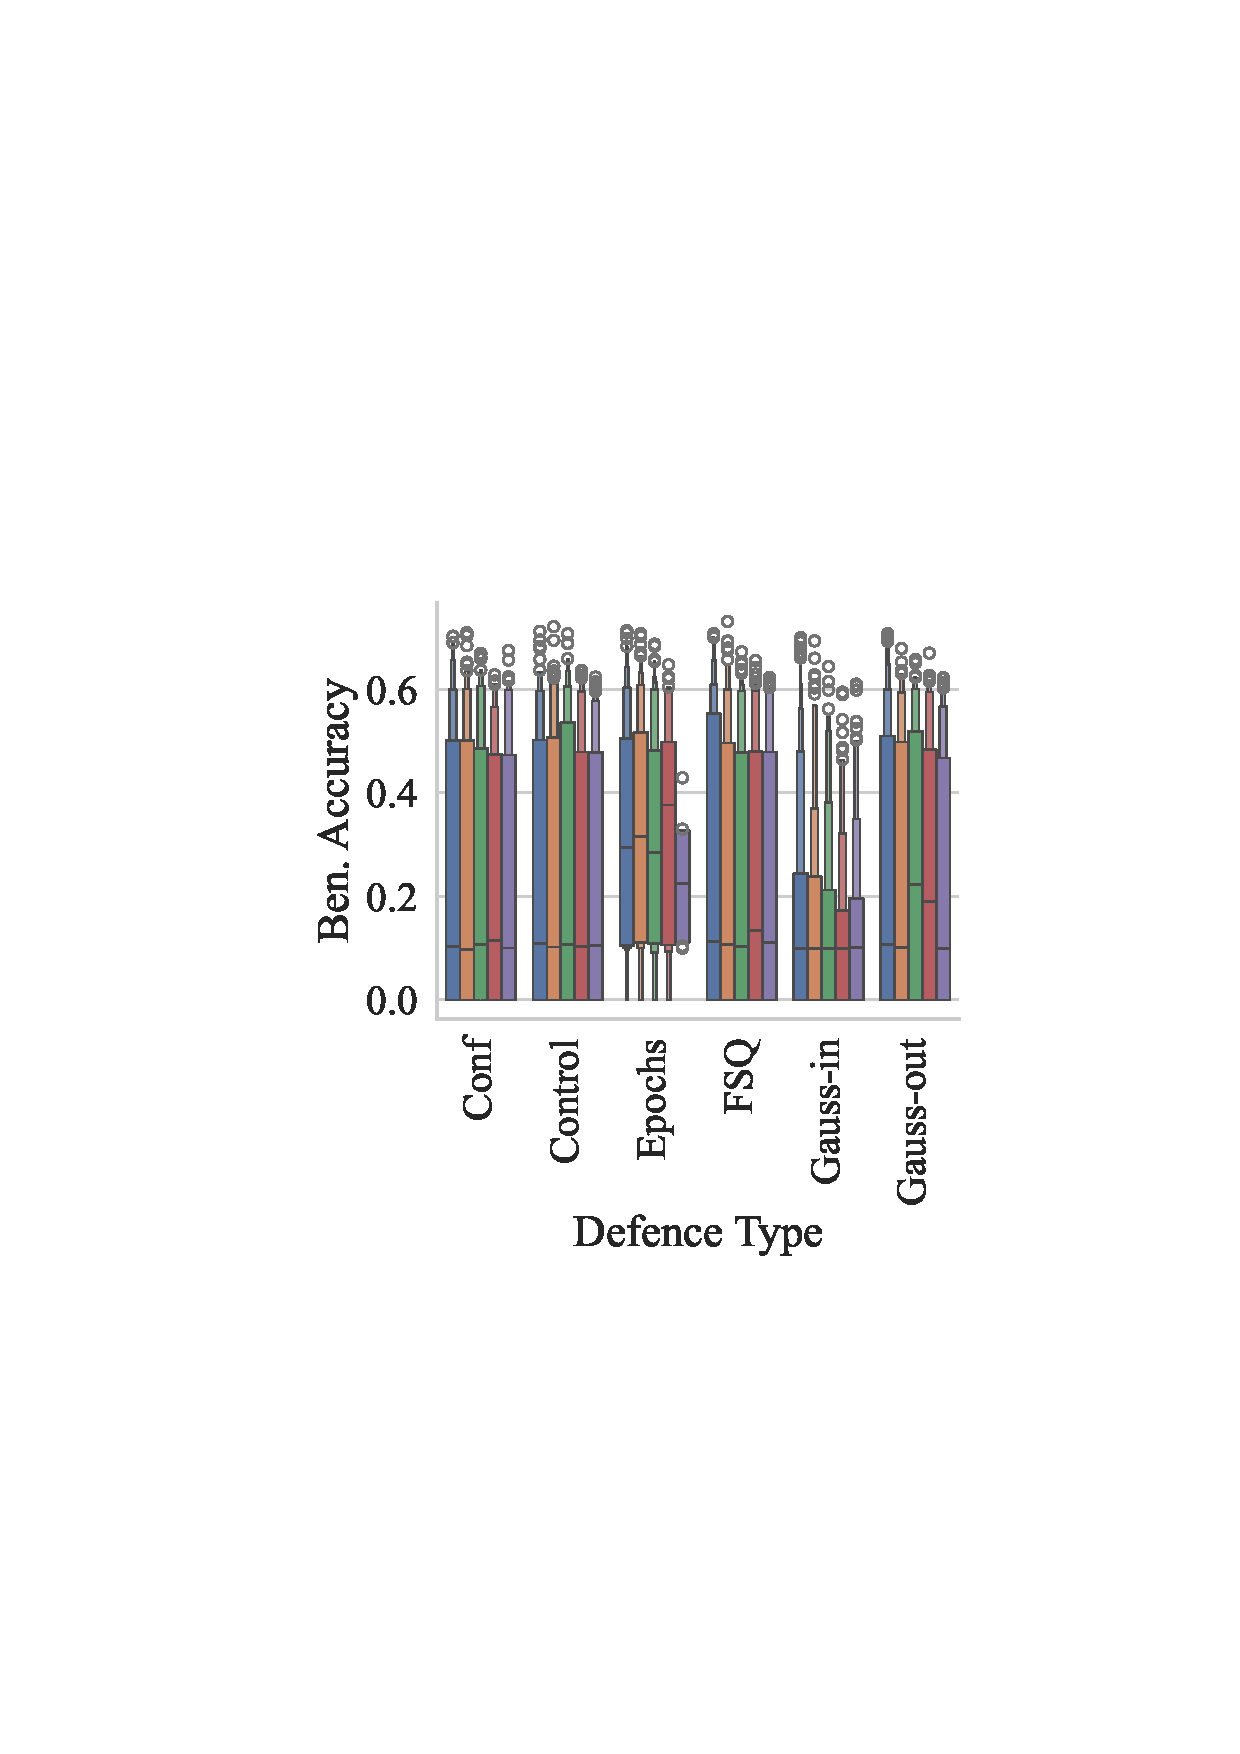
\includegraphics[trim={0 5pt 0 10pt},clip,width=.45\textwidth]{plots/ben_accuracy_vs_defence_type.pdf}
\end{subfigure}
\begin{subfigure}
    \centering
    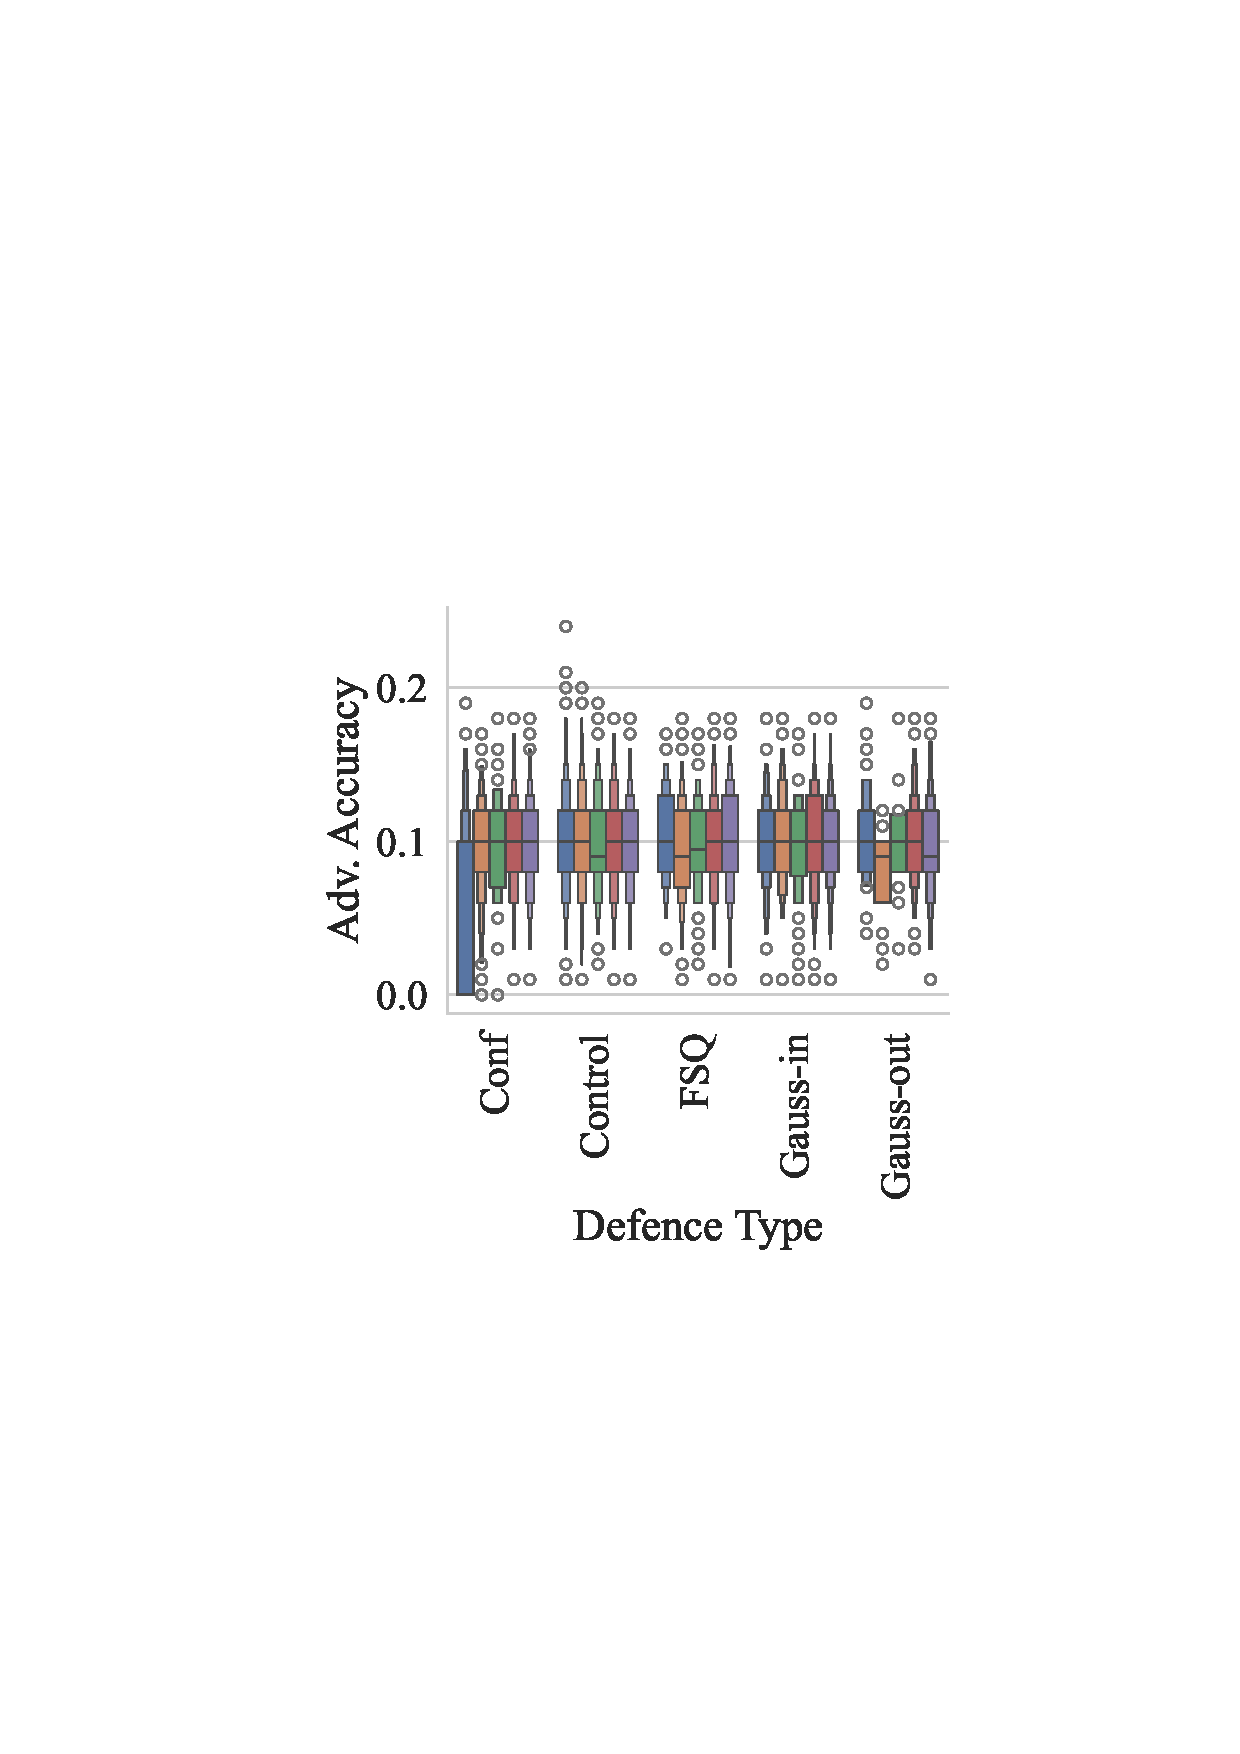
\includegraphics[trim={0 5pt 0 10pt},clip,width=.45\textwidth]{plots/adv_accuracy_vs_defence_type.pdf}
\end{subfigure}
\begin{subfigure}
    \centering
    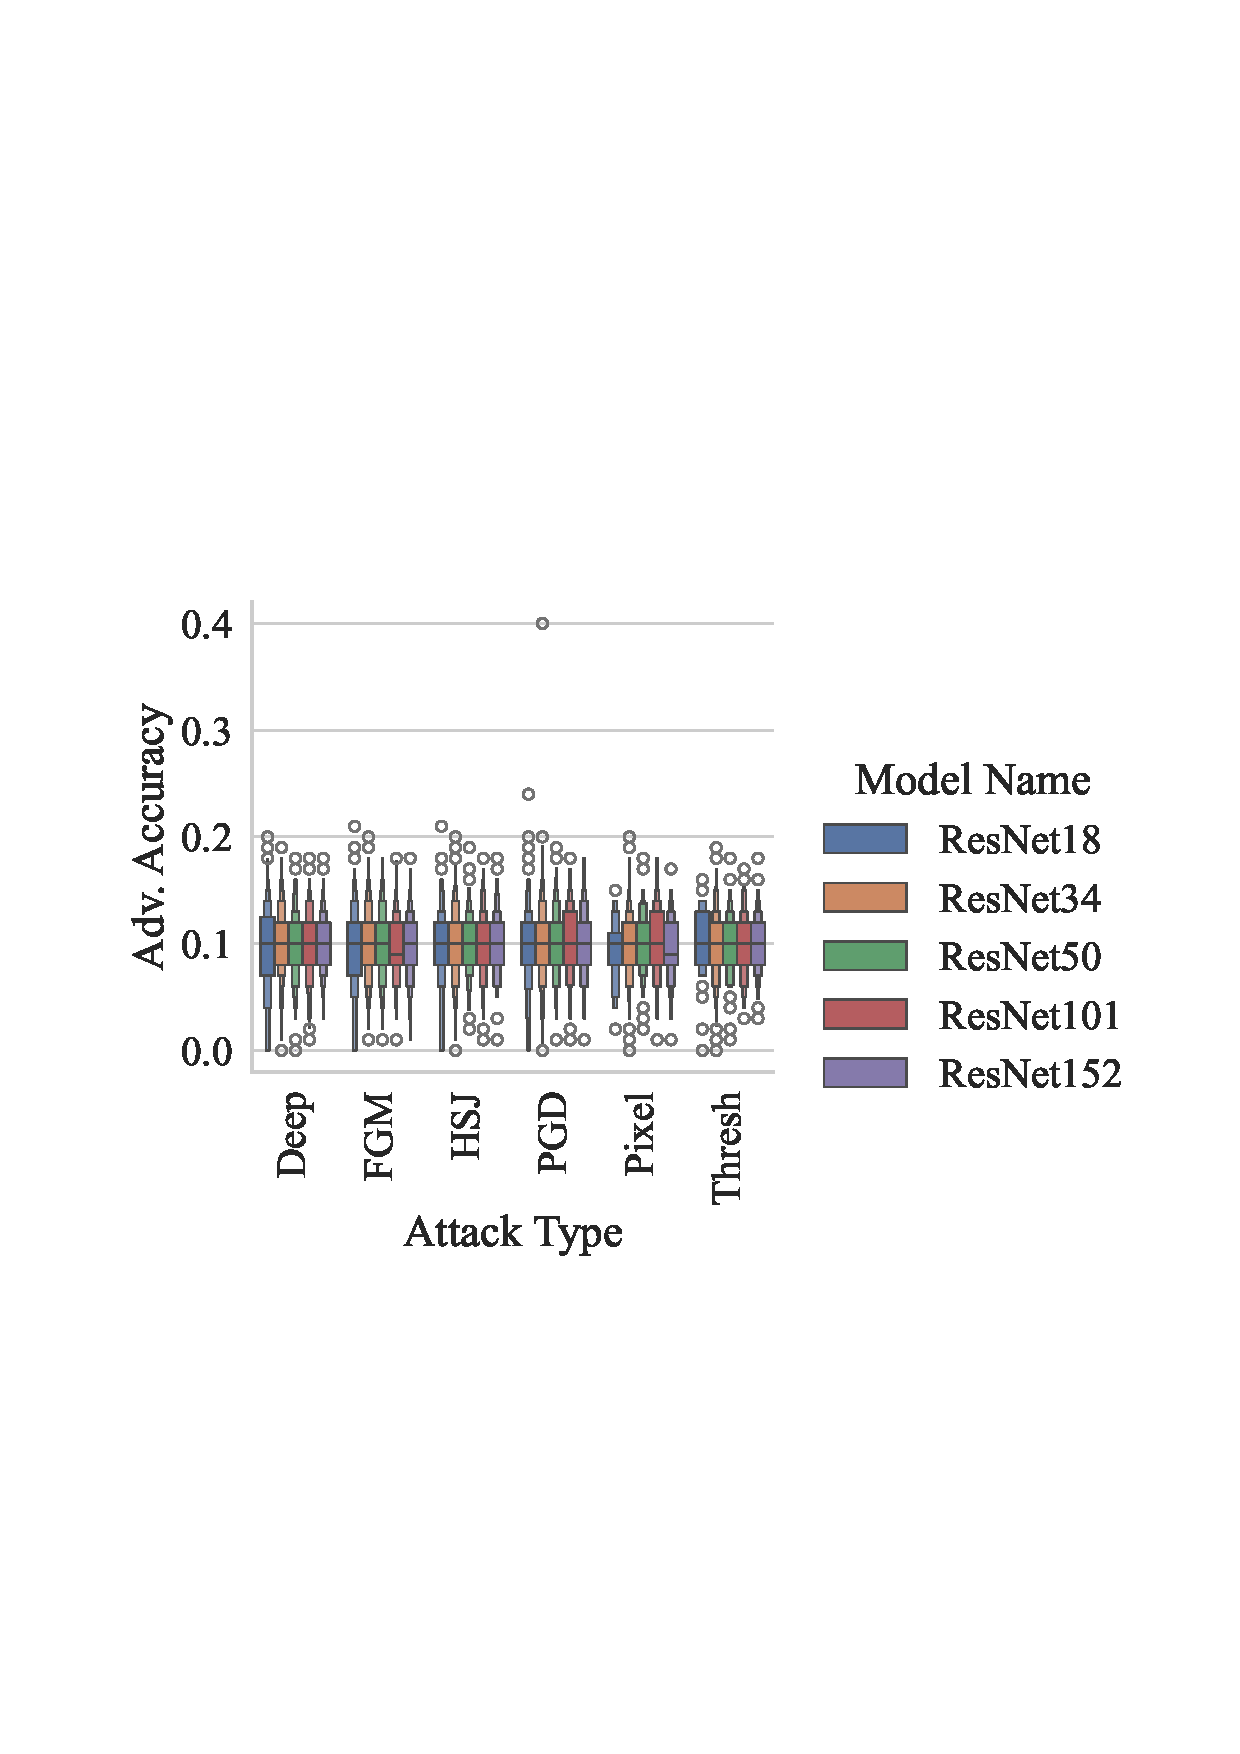
\includegraphics[trim={0 5pt 0 10pt},clip,width=.45\textwidth]{plots/adv_accuracy_vs_attack_type.pdf}
\end{subfigure}
\caption{The adversarial accuracy across various attacks pictured on the x-axis and outlined in Section~\ref{attacks}. The error bar reflects the 95\% confidence interval for the adversarial accuracy across all examined samples. The violin plots reflect the 95\% confidence intervals for each tuned hyperparameter combination. Outliers are indicated with a circle.}
\label{fig:accuracies}
\end{figure}

\begin{figure}[!h]
    \centering
    \begin{subfigure}
        \centering
        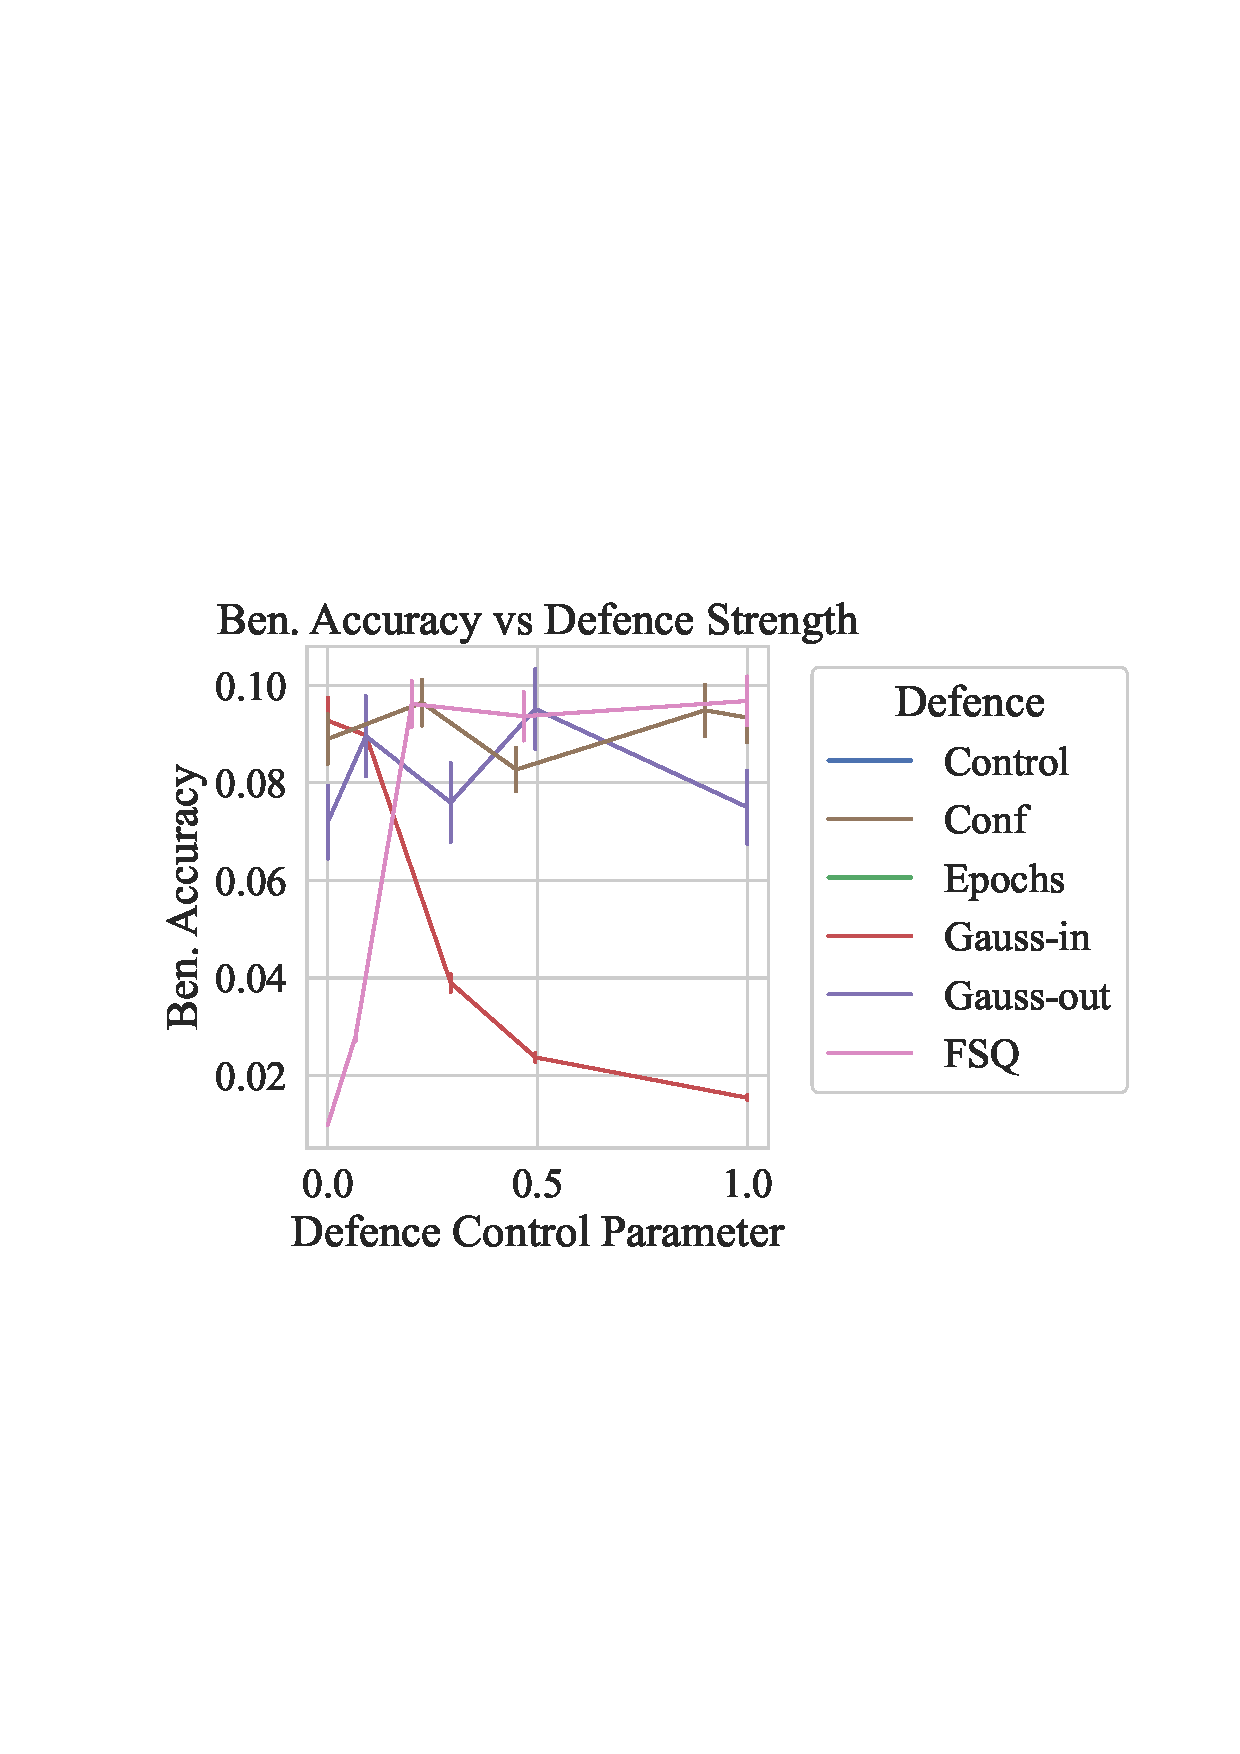
\includegraphics[trim={0 10pt 0 10pt},clip,width=.45\textwidth]{plots/def_param_vs_accuracy.pdf}
    \end{subfigure}
    \begin{subfigure}
        \centering
        \includegraphics[trim={0 10pt 0 10pt},clip,width=.45\textwidth]{plots/atk_param_vs_accuracy.pdf}
    \end{subfigure}
    \caption{This depicts the benign (unperturbed) and adversarial (perturbed) failure rates across all defences attacks, and models. The left shows how the benign accuracy varies with the defence strength where the control parameter describes the number of layers. The right shows the adversarial accuracy as a function of attack strength. The bars indicate the first standard deviation of measures across all model configurations.}
    \label{fig:strength}
\end{figure}

% \begin{figure}[!h]
%     \centering
%     \begin{subfigure}
%         \centering
%         \includegraphics[width=.4\textwidth]{plots/def_param_vs_adv_failure_rate.pdf}
%     \end{subfigure}
%     \begin{subfigure}
%         \centering
%         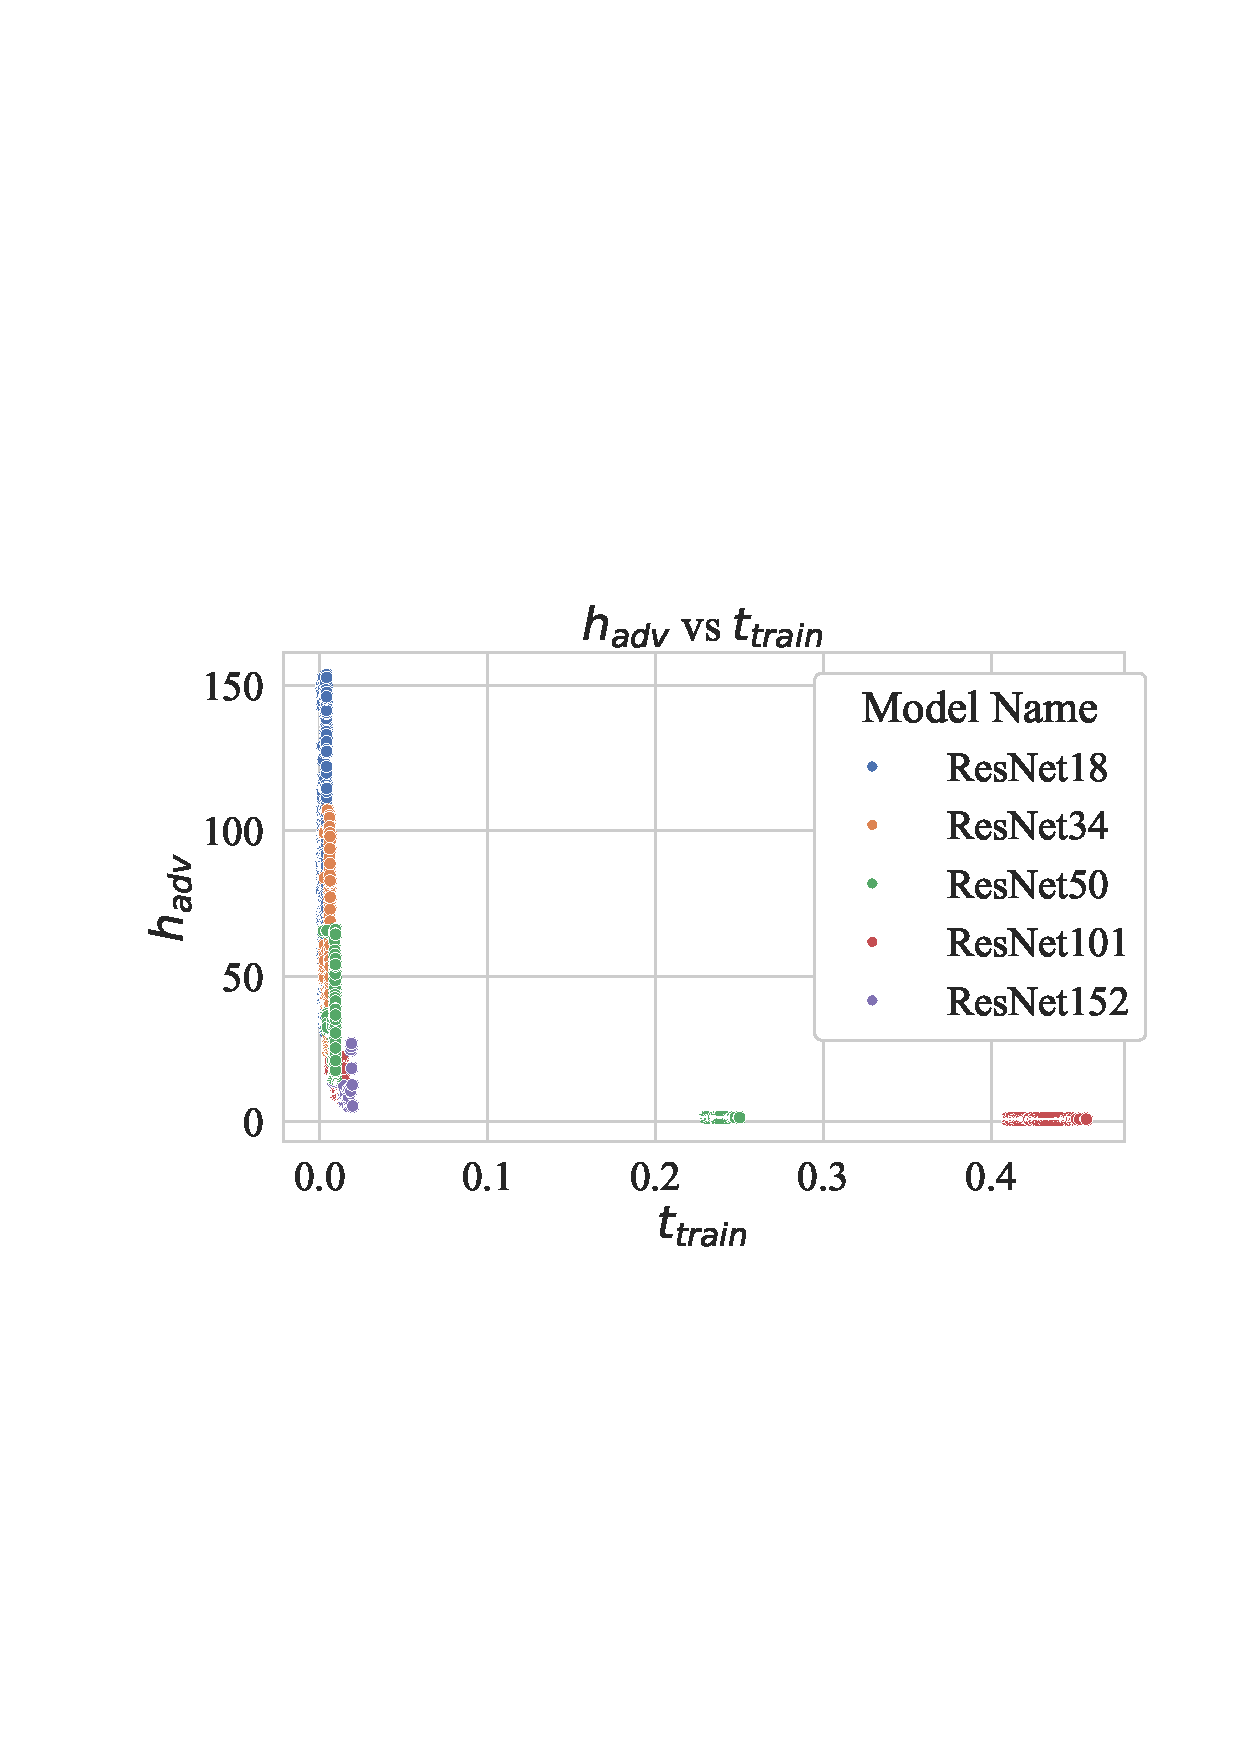
\includegraphics[width=.4\textwidth]{plots/adv_failure_rate_vs_train_time.pdf}
%     \end{subfigure}
%     \caption{The left shows the adversarial failure rate as a function of the defence strength where the control parameter represents the number of model layers. The right depicts the adversarial failure rate as a function of training time and the ResNet configuration. The bars indicate the first standard deviation of measures across all model configurations.}
%     \label{fig:failure_rate}
% \end{figure}

\begin{figure}[!h]
    \centering
    \begin{subfigure}
        \centering
        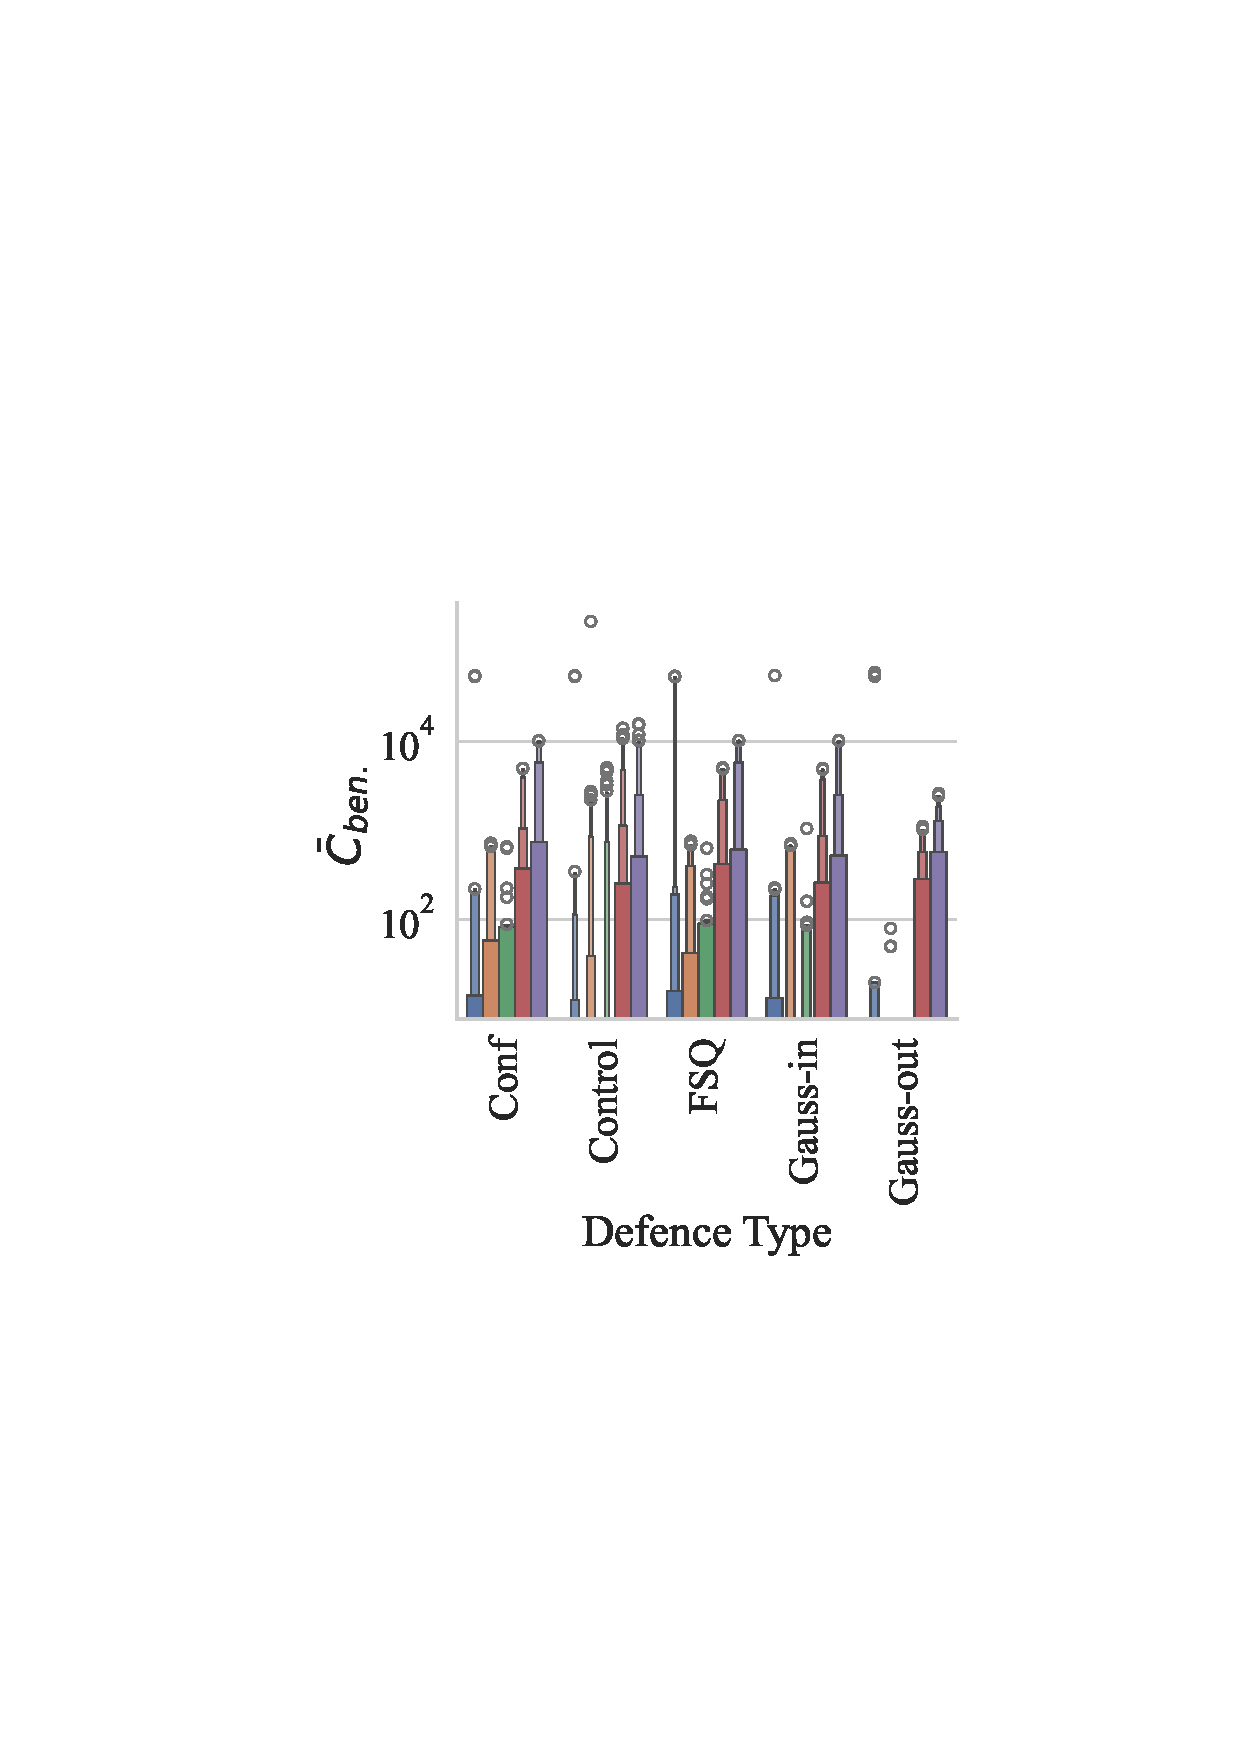
\includegraphics[width=.45\textwidth]{plots/ben_failures_per_train_time_vs_defence_type.pdf}
    \end{subfigure}
    \begin{subfigure}
        \centering
        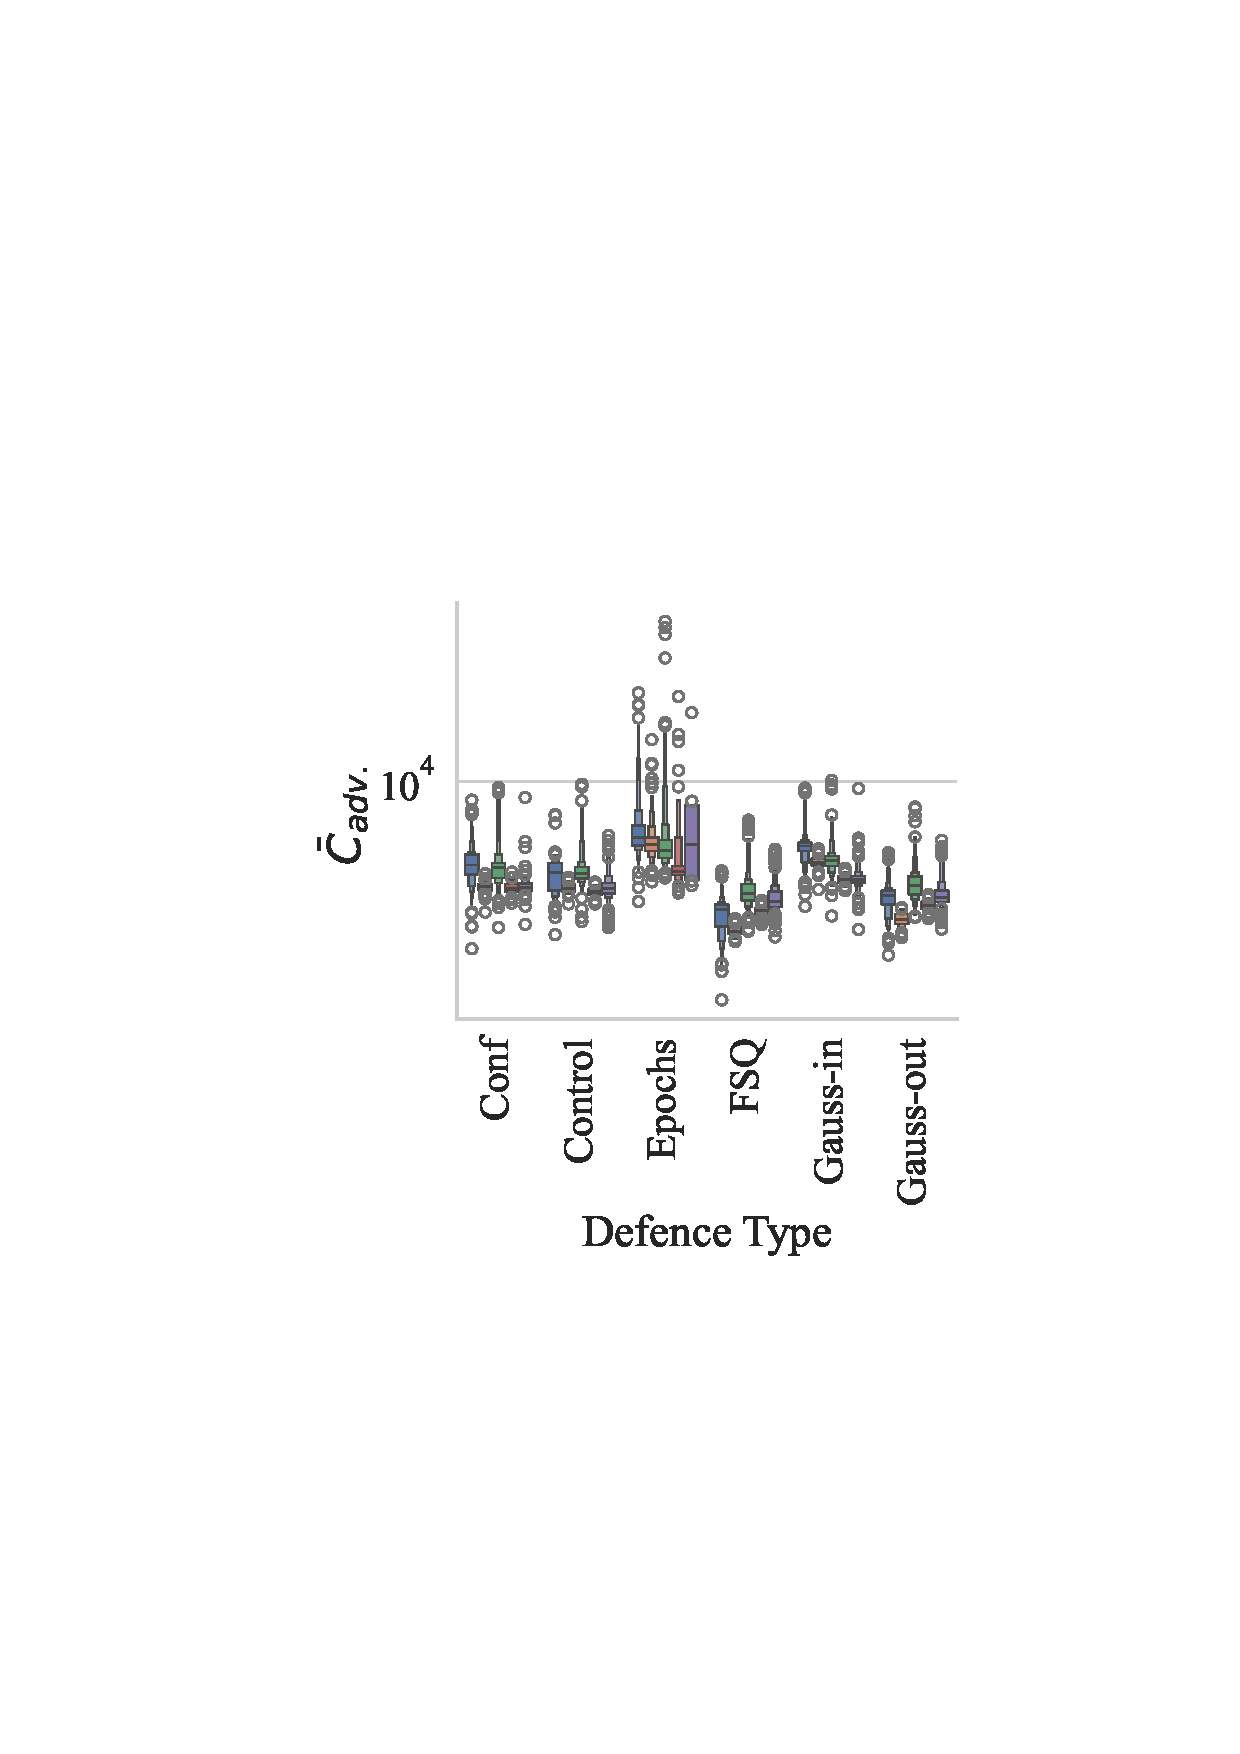
\includegraphics[width=.45\textwidth]{plots/adv_failures_per_train_time_vs_defence_type.pdf}
    \end{subfigure}
    \begin{subfigure}
        \centering
        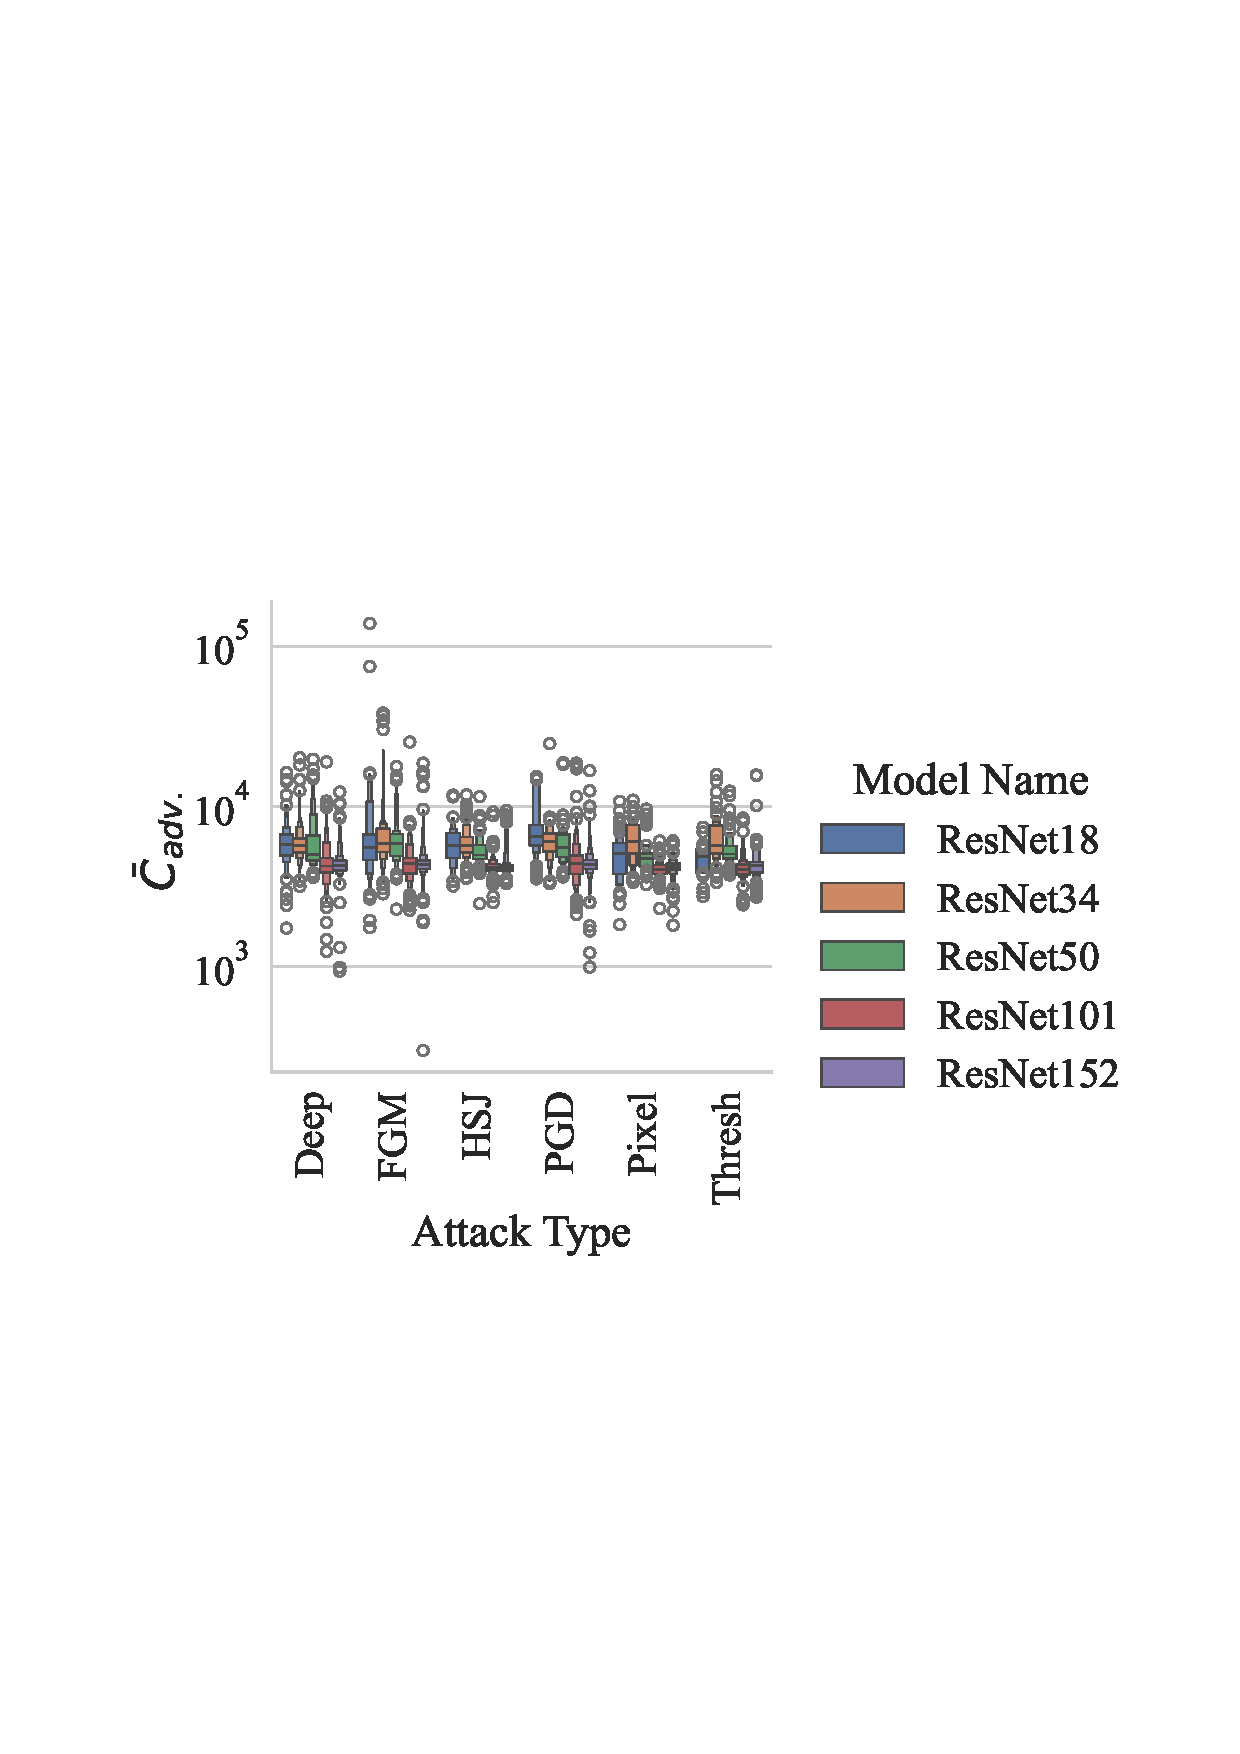
\includegraphics[width=.45\textwidth]{plots/adv_failures_per_train_time_vs_attack_type.pdf}
    \end{subfigure}
    \caption{This figure depicts the cost-normalized adversarial failure rate across a variety of defences and attacks, where training time (middle~\&~right Figs.) and inference time (left figure) is a stand-in for cost (see Section~\ref{cost}). The violin plots reflect the 95\% confidence intervals for each tuned hyperparameter combination. Outliers are indicated with a circle.}
    \label{fig:failures_per_train_time}
\end{figure}


Through tens of thousands experiments across many signal-processing techniques (\textit{e.g.}, defences), random states, learning rates, model architectures, and attack configurations, we show that model defences generally fail to outperform the undefended model in either the benign or adversarial contexts--- regardless of configuration; that the adversarial failure rate gains of larger ResNet configurations are driven by response time rather than true robustness; that these gains are dwarfed by the increase in training time; and that AFR models are a powerful tool for comparing model architectures and examining the effects of covariates. In the section below, we display and discuss the results for the CIFAR100, CIFAR10, and MNIST datasets for all attacks and defences. Fig.~\ref{fig:accuracies} depicts the benign and adversarial accuracies across the various attacks and defences. We can clearly see that no defence consistently outperforms the undefended (control) model in either the benign (top) or adversarial context (middle).



% \subsection{Attack and Defence Strength}
% In Fig.~\ref{fig:strength},  (denoted in blue). Furthermore, the relationship between the defence control parameter and the benign accuracy is not monotonic, meaning that tuning is will be expensive. We can see that the relationship between the attack parameters and failure rate is also not monotonic. However, all defences appear to perform much worse in the average adversarial case (right) than in the benign (left). Additionally we see in the right side of Fig.~\ref{fig:strength} that the attack types yield relatively consistent results, with the mean of one falling in the 95 confidence intervals of all the others. We can also see that defence choice follows the same pattern, except for Gauss-in, which rapidly decreases the accuracy as we increase the input noise.


% \subsection{Failure Rate}
% Fig.~\ref{fig:failure_rate} depicts the adversarial failure rate of all tested attacks, defences, and model configurations. 
% Clearly, increasing the depth of the model architecture does little for adversarial robustness while universally increasing the training time. 
% Furthermore, it reveals something surprising---that increasing the number of hidden layers tends to increase the failure rate---even across model architectures and all defences. 
% Certain defences can outperform the control model---at the cost of expensive tuning---evidenced by the large variance in performance (see left side of Fig.~\ref{fig:failure_rate}). The right subplot of Fig.~\ref{fig:failure_rate} shows that there is no general relationship between training time and adversarial failure rate.
% As the training time increases, however, the variance of attack times decreases, likely due to the increase in inference time (see:~\ref{fig:afr_models}) rather than inherent robustness.
% We formalize this analysis  in the next subsection.

Fig.~\ref{fig:failures_per_train_time} depicts the cost-normalized failure rate in both the benign (left) figure and adversarial cases (middle and right figures). Counter-intuitively, we see that the smallest model (ResNet18) tends to outperform both larger models (ResNet50 and ResNet152). Furthermore, we see that defence tuning is about as important as choosing the right type of defence (see: left side of Fig.~\ref{fig:failures_per_train_time}), with all defences falling within the normal ranges of each other. However, adding noise to the model output (Gauss-out) tends to underperform relative to the control for all models (see: left side of Fig.~\ref{fig:failures_per_train_time}). Likewise, the intersectional relationship between model choice and optimal defence is highlighted since the efficacy of a defence depends as much on model architecture as it does on hyperparameter tuning.  Furthermore, performance across all attacks is remarkably consistent with intra-class variation being smaller than inter-class variation almost universally across defences and model configurations.



\subsection{AFR Models}

Fig.~\ref{fig:afr_models} reveals very similar estimates for the model parameters despite the models having different forms, suggesting that these parameter estimates reflect the true effect of these covariates on the failure rate. Table~\ref{tab:combined} contains the performance of each of these models on the CIFAR10 dataset. For all datasets, we can see that they are roughly comparable with regards to Concordance, but that Log-Normal model marginally outperforms the Weibull model when measured with AIC/BIC as well as the Concordance.
In all cases, the mean time until false classification is much larger than the median, indicating the long-tailed nature of these distributions.
The concordance scores for all three distributions are in agreement as well, confirming our assumption that accuracy is not independent of attack time (e.g., Concordance $> 0.5$).
We then used the Log-Normal AFR to demonstrate the partial effect of the the number of layers on the survival time as in Fig.~\ref{fig:covariates}. In that figure can clearly see that more hidden layers do increase the survival time. However, that seems to driven more by the model query time (see Fig.~\ref{fig:afr_models}) than the number of model layers.
\begin{figure*}
	% \centering
	\begin{subfigure}
		\centering
		\includegraphics[width=.32\textwidth]{plots/weibull_qq.pdf}
	\end{subfigure}%
	~
	\begin{subfigure}
		\centering
		\includegraphics[width=.32\textwidth]{plots/log_normal_qq.pdf}
	\end{subfigure}
	~
	\begin{subfigure}
		\centering
		\includegraphics[width=.32\textwidth]{plots/log_logistic_qq.pdf}
	\end{subfigure}
 \begin{subfigure}
		\centering
		\includegraphics[width=.32\textwidth]{plots/exponential_qq.pdf}
	\end{subfigure}%
	~
	\begin{subfigure}
		\centering
		\includegraphics[width=.32\textwidth]{plots/gamma_qq.pdf}
	\end{subfigure}
	~
	\begin{subfigure}
		\centering
		\includegraphics[width=.32\textwidth]{plots/cox_qq.pdf}
	\end{subfigure}
	\caption{These quantile-quantile plots demonstrate the efficacy of various AFR models. The x-axis is the observed p-value of a sample and the y-axis represents the theoretical p-value according to the chosen AFR model. The dashed black line represents a perfect fit. To verify each model, we reserved 80\% of the data to be the training set (red) and 20\% to be the test set (blue). The absence of one of the lines means that the \texttt{lifelines} fitter failed to converge for that subset.}
	\label{fig:afr_models}
\end{figure*}
\begin{table*}
\centering
\label{tab:afr_models}
\begin{tabular}{lllrrrrrr}
\toprule
 & AIC & BIC & Concordance & Test Concordance & ICI & Test ICI & E50 & Test E50 \\
\midrule
Weibull & 9.05e+04 & 9.05e+04 & 0.92 & 0.92 & 0.02 & 0.02 & 0 & 0 \\
Cox & -- & -- & 0.92 & 0.92 & 0.09 & 0.08 & 0.09 & 0.04 \\
Log Logistic & 8.76e+04 & 8.76e+04 & 0.92 & 0.92 & 0.03 & 0.03 & 0.01 & 0.01 \\
Log Normal & 1.14e+05 & 1.14e+05 & 0.91 & 0.91 & 0.15 & 0.08 & 0.08 & 0.01 \\
Gamma & 9.99e+04 & 9.99e+04 & 0.52 & 0.52 & 0.26 & 0.15 & 0.19 & 0.13 \\
Exponential & 7.93e+04 & 7.93e+04 & 0.86 & 0.86 & 0.03 & 0.04 & 0 & 0 \\
\bottomrule
\end{tabular}
\end{table*}

\begin{figure}
    \centering
	\begin{subfigure}
	\centering
    \includegraphics[width=.38\textwidth]{plots/weibull_aft_dummies.pdf}
    \label{fig:covariates}
    \end{subfigure}
    \begin{subfigure}
	\centering
    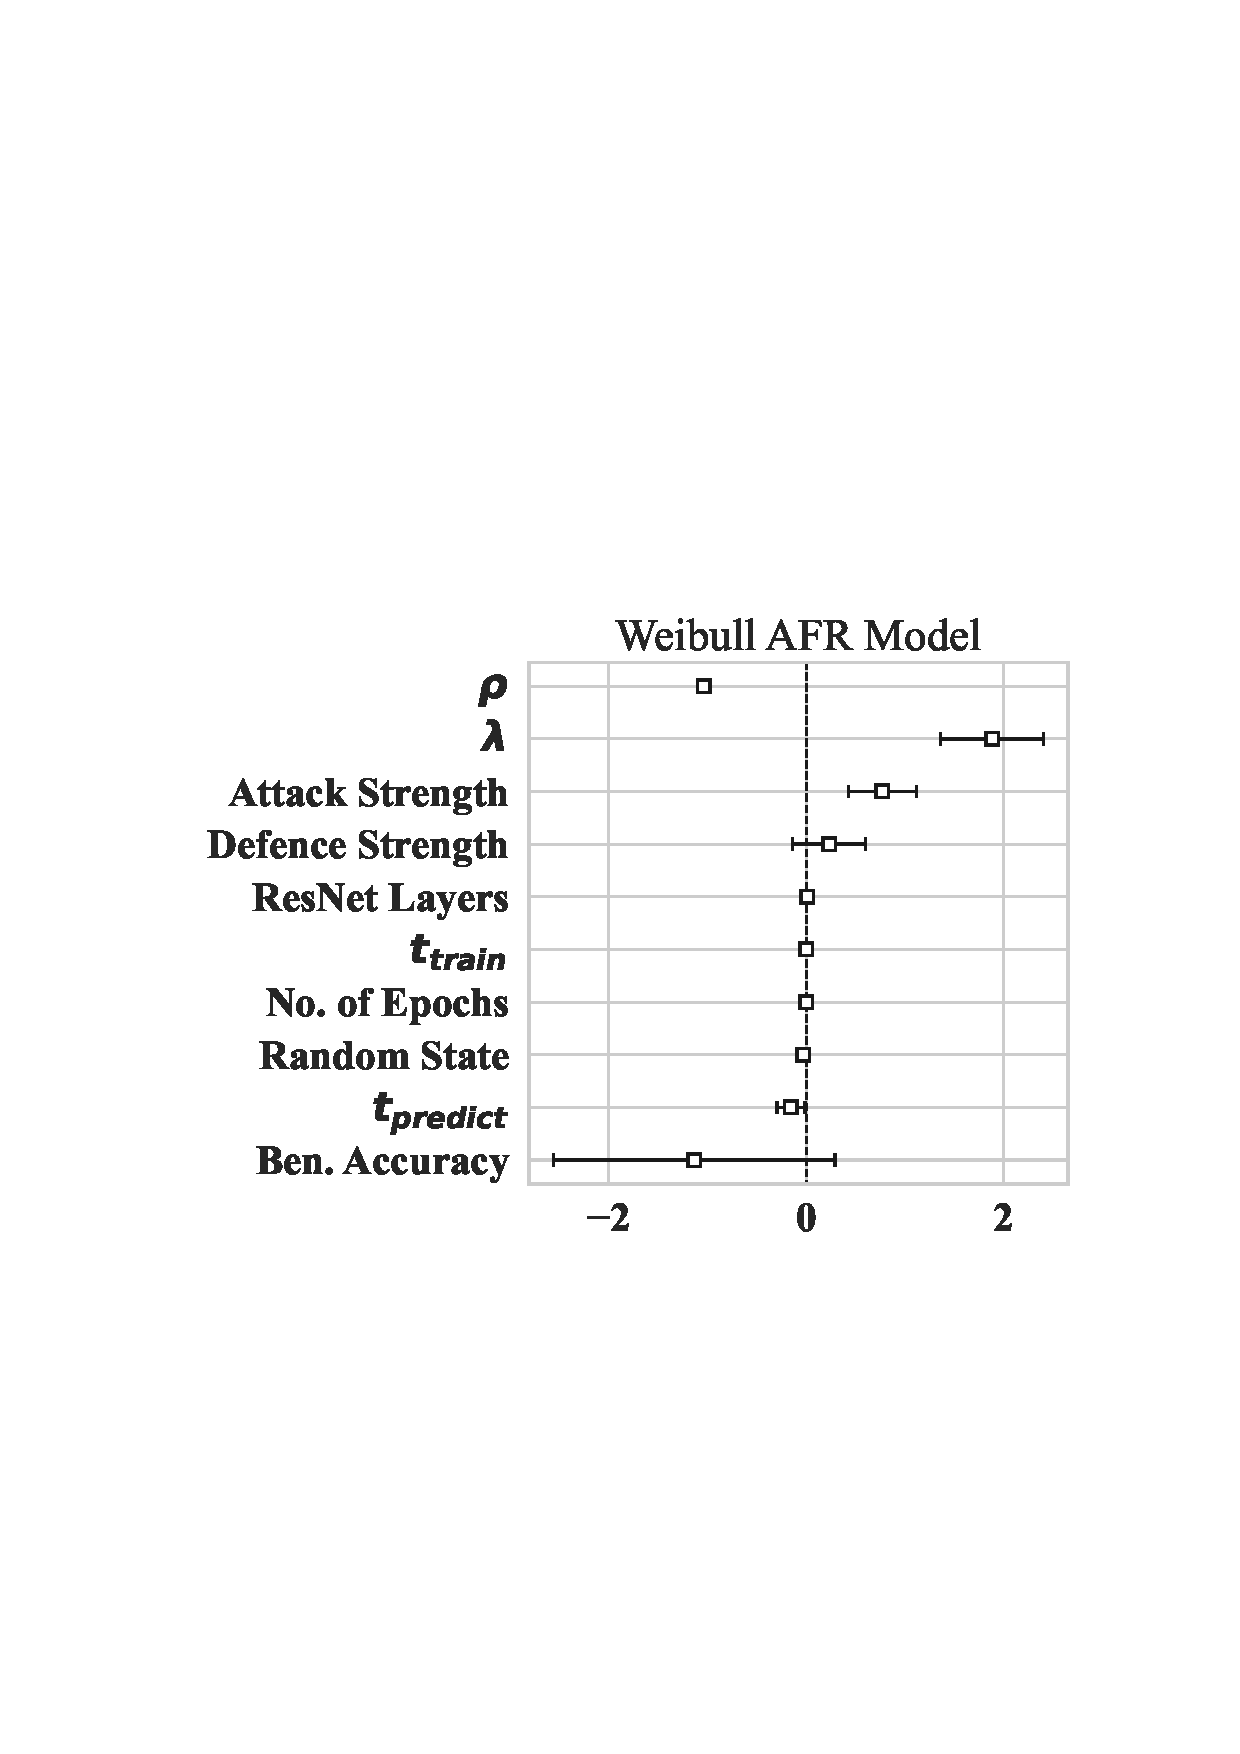
\includegraphics[width=.38\textwidth]{plots/weibull_aft.pdf}
    \label{fig:dummies}
    \end{subfigure}
    \caption{The coefficients represent the log scale effect of the dummy variables for dataset, attack, and defence on the survival time, with a positive value indicating an increase in the survival time.}
\end{figure}




\section{Considerations}
The proposed survival and cost analysis  has some limitations that we have taken all efforts to minimise and/or mitigate. 
In order to minimise timing jitter, we measured the process time for a batch of samples and then assumed that the time per sample was the measured processor time divided by the number of samples. 
In order to examine a variety of different optimisation criteria for adversarial perturbations, we included several different attacks (see Section~\ref{attacks})---though the choice of attack is highly contextual.
We must also note that none of these attacks are run-time optimal and are, at best, an underestimate of the true adversarial failure rate~\cite{meyers}. 
Likewise, testing all known defences would be computationally infeasible. 
As such, we focused only on the pre- and post-processing technique. 
% Techniques like adversarial retraining~\cite{croce_reliable_2020}, model transformation~\cite{papernot_distillation_2016}, and model regularisation~\cite{jakubovitz2018improving} were excluded due to their comparatively larger run-times. The equation Section~\ref{cost_normalization} reveals why techniques that significantly increase the training time might ultimately work against the model builder.
% Even if one assumes there is a defence that has 99\% efficacy, rather than the, at best, 40\% efficacy indicated by the adversarial accuracy in Figure~\ref{fig:accuracies}, it would only reduce $\bar{C}_{\mathrm{adv}}$ by roughly two orders of magnitude.
While every configuration of ResNet met the bare minimum requirement outlined in Equation~\ref{eq:cost}, real training processes require many thousands of samples and attacks are consistently successful with only one hundred samples. 
Together, these considerations raise serious concerns about the efficacy of any of these models and defences in the presence of these simple adversaries, meaning attacks will likely be many orders of magnitude cheaper than defences for tested configurations of this model.
Furthermore, state of-the art leaderboards\footnote{\href{https://github.com/MadryLab/mnist\_challenge}{Madry's MNIST Challenge}}\footnote{\href{https://ml.cs.tsinghua.edu.cn/adv\-bench/}{Croce's Robust Bench}}
show that a 99\% generalised adversarial accuracy is, at best, optimistic. 
% Nevertheless, the goal of this work was not to produce a comprehensive evaluation of all known defences, but to develop a cost-aware framework for evaluating their efficacy against a set of adversaries.

\section{Conclusion}
Convolutional neural networks have shown to be widely applicable to a large number of fields when large amounts of labelled data are available.
By examining the role of the attacks, defences, and model depth in the context of adversarial failure rate, this paper presents a reliable and effective modelling framework that applies AFT models to deep neural networks.
The metrics outlined Table~\ref{tab:aft_summary} and explained in Section~\ref{metrics} show that this method is both effective and data-agnostic.  
We use this model to demonstrate the efficacy of various attack- and defence-tuning techniques, to  explore the relationships between accuracy and adversarial robustness (Figure~\ref{fig:dummies}), and show that various model defences are ineffective on average and marginally better than the control at best.
By measuring the cost-normalised failure rate or TRASH score (see Section~\ref{cost_normalization} and Figure~\ref{fig:trash}), it is clear that all tested configurations of ResNet fail to meet the TRASH criterion.
The methods can easily extend to any other arbitrary collection of model pre-processing, training, tuning, attack and/or deployment parameters. 
In short, AFTs provide a rigorous way to compare not only the relative robustness of a model, but of its cost effectiveness in response to an attacker.
The measurements rigorously demonstrate  that the depth of a ResNet architecture does little to guarantee robustness while the community trends towards larger models~\cite{desislavov2021compute}. 

While the train-test split methodology relies on an ever-larger number of samples to increase precision, the survival time method is able to precisely and accurately compare models using only a small number of samples~\cite{schmoor2000sample,lachin1981introduction} relative to the many billions of samples required of the train/test split methodology and safety-critical standards~\cite{iso26262,IEC61508,IEC62034,meyers}.
In short, by generating worst-case examples (\textit{e.g.}, adversarial ones), one can test and compare arbitrarily complex models \textit{before} they leave the lab, drive a car, predict the presence of cancer, or pilot a drone.

\printbibliography
\end{document}

